% SkinCare AI - CMP6200 Final Report
% Compile: tectonic main.tex   (XeLaTeX engine; Arial must be installed)
% Layout follows the BCU final report template (final_report_template.docx).
\documentclass[11pt,a4paper]{article}
\usepackage{fontspec}
\setmainfont{Arial}[Ligatures=NoCommon]
\setmonofont{Menlo}[Scale=0.85]
\usepackage[
  paperwidth=595.5bp,paperheight=842bp,
  left=72bp,right=72bp,top=100bp,bottom=72bp,
  headheight=34bp,headsep=24bp
]{geometry}
\usepackage{fancyhdr}
\usepackage{graphicx}
\usepackage{tikz}
\usetikzlibrary{positioning,arrows.meta,fit,backgrounds,calc,shapes.geometric}
\usepackage{pgfplots}
\pgfplotsset{compat=1.18}
\pgfkeys{/pgf/number format/assume math mode=true}
\usepackage{pgfgantt}
\usepackage{enumitem}
\usepackage{needspace}
\usepackage{booktabs,tabularx,multirow,longtable,array}
\usepackage{xcolor}
\usepackage[font=small,labelfont=bf]{caption}
\usepackage{subcaption}
\usepackage{listings}
\usepackage{titlesec}
\usepackage[titles]{tocloft}
\usepackage[round]{natbib}
\usepackage[hidelinks]{hyperref}
\usepackage{amsmath,amssymb}

\definecolor{TemplateBlue}{HTML}{0E2841}
\definecolor{Accent}{HTML}{C2185B}
\definecolor{AccentLight}{HTML}{F8D7E3}
\definecolor{Muted}{HTML}{5F6B7A}
\definecolor{BoxA}{HTML}{E8F0FB}
\definecolor{BoxB}{HTML}{E6F4EA}
\definecolor{BoxC}{HTML}{F1EAFB}
\definecolor{BoxD}{HTML}{FDF1E0}

% BEGIN EMBEDDED TEMPLATE LOGO
\newcommand{\TemplateLogo}{%
  \resizebox{155.03bp}{32.03bp}{%
    
\begin{tikzpicture}[x=1bp,y=1bp]
      \useasboundingbox (0,0) rectangle (523,107);
      \path[fill=black!90,draw=none]
        (34,104) rectangle (36,105)
        (33,103) rectangle (36,104)
        (49,101) rectangle (50,102)
        (30,100) rectangle (36,103)
        (47,100) rectangle (50,101)
        (30,99) rectangle (35,100)
        (37,99) rectangle (40,100)
        (44,99) rectangle (50,100)
        (18,98) rectangle (23,99)
        (89,98) rectangle (90,99)
        (76,98) rectangle (80,99)
        (30,98) rectangle (34,99)
        (36,98) rectangle (50,99)
        (74,97) rectangle (84,98)
        (88,97) rectangle (89,98)
        (17,97) rectangle (49,98)
        (15,96) rectangle (49,97)
        (5,96) rectangle (10,97)
        (72,95) rectangle (89,97)
        (4,95) rectangle (48,96)
        (71,94) rectangle (88,95)
        (4,94) rectangle (47,95)
        (4,93) rectangle (46,94)
        (71,93) rectangle (87,94)
        (29,92) rectangle (44,93)
        (3,92) rectangle (21,93)
        (70,92) rectangle (85,93)
        (3,91) rectangle (23,92)
        (70,91) rectangle (82,92)
        (30,91) rectangle (44,92)
        (69,90) rectangle (81,91)
        (3,90) rectangle (24,91)
        (29,90) rectangle (45,91)
        (68,89) rectangle (81,90)
        (4,88) rectangle (47,90)
        (67,88) rectangle (80,89)
        (184,87) rectangle (199,88)
        (67,87) rectangle (77,88)
        (13,87) rectangle (48,88)
        (303,87) rectangle (311,88)
        (440,87) rectangle (447,88)
        (497,87) rectangle (502,88)
        (326,87) rectangle (330,88)
        (214,87) rectangle (219,88)
        (142,87) rectangle (157,88)
        (264,87) rectangle (268,88)
        (365,87) rectangle (369,88)
        (238,87) rectangle (243,88)
        (385,87) rectangle (390,88)
        (409,86) rectangle (414,88)
        (516,86) rectangle (521,88)
        (497,86) rectangle (503,87)
        (15,86) rectangle (48,87)
        (301,86) rectangle (313,87)
        (264,86) rectangle (269,87)
        (437,86) rectangle (450,87)
        (365,86) rectangle (370,87)
        (184,86) rectangle (203,87)
        (142,86) rectangle (160,87)
        (66,86) rectangle (73,87)
        (385,85) rectangle (391,87)
        (436,85) rectangle (450,86)
        (8,85) rectangle (12,86)
        (300,85) rectangle (315,86)
        (184,85) rectangle (204,86)
        (498,85) rectangle (503,86)
        (142,85) rectangle (161,86)
        (16,85) rectangle (48,86)
        (515,85) rectangle (521,86)
        (65,85) rectangle (71,86)
        (214,84) rectangle (220,87)
        (237,84) rectangle (243,87)
        (364,84) rectangle (370,86)
        (264,84) rectangle (270,86)
        (408,84) rectangle (414,86)
        (184,84) rectangle (205,85)
        (498,84) rectangle (504,85)
        (515,84) rectangle (520,85)
        (6,84) rectangle (11,85)
        (434,84) rectangle (452,85)
        (65,84) rectangle (69,85)
        (298,84) rectangle (316,85)
        (471,83) rectangle (494,88)
        (385,83) rectangle (392,85)
        (142,83) rectangle (163,85)
        (17,83) rectangle (49,85)
        (298,83) rectangle (317,84)
        (5,83) rectangle (9,84)
        (433,83) rectangle (453,84)
        (184,83) rectangle (206,84)
        (264,83) rectangle (271,84)
        (499,83) rectangle (504,84)
        (514,82) rectangle (519,84)
        (65,82) rectangle (68,84)
        (236,82) rectangle (243,84)
        (214,82) rectangle (221,84)
        (200,82) rectangle (207,83)
        (297,82) rectangle (304,83)
        (2,82) rectangle (8,83)
        (45,82) rectangle (49,83)
        (447,82) rectangle (453,83)
        (311,82) rectangle (317,83)
        (499,82) rectangle (505,83)
        (97,82) rectangle (104,83)
        (157,82) rectangle (164,83)
        (17,82) rectangle (44,83)
        (433,82) rectangle (440,83)
        (407,81) rectangle (414,84)
        (363,81) rectangle (371,84)
        (264,81) rectangle (272,83)
        (500,81) rectangle (505,82)
        (3,81) rectangle (7,82)
        (158,81) rectangle (164,82)
        (94,81) rectangle (106,82)
        (448,81) rectangle (454,82)
        (513,81) rectangle (519,82)
        (201,81) rectangle (207,82)
        (312,81) rectangle (318,82)
        (296,81) rectangle (303,82)
        (385,80) rectangle (393,83)
        (235,80) rectangle (243,82)
        (47,80) rectangle (49,82)
        (65,80) rectangle (69,82)
        (214,80) rectangle (222,82)
        (17,80) rectangle (43,82)
        (432,80) rectangle (438,82)
        (264,80) rectangle (273,81)
        (296,80) rectangle (302,81)
        (313,80) rectangle (318,81)
        (92,80) rectangle (108,81)
        (500,80) rectangle (506,81)
        (363,80) rectangle (372,81)
        (513,80) rectangle (518,81)
        (406,79) rectangle (414,81)
        (449,79) rectangle (454,81)
        (8,79) rectangle (46,80)
        (501,79) rectangle (506,80)
        (512,79) rectangle (518,80)
        (362,79) rectangle (372,80)
        (90,79) rectangle (110,80)
        (313,79) rectangle (319,80)
        (432,78) rectangle (437,80)
        (65,78) rectangle (70,80)
        (214,78) rectangle (223,80)
        (385,78) rectangle (394,80)
        (264,78) rectangle (274,80)
        (234,78) rectangle (243,80)
        (362,78) rectangle (367,79)
        (8,78) rectangle (49,79)
        (88,78) rectangle (97,79)
        (512,78) rectangle (517,79)
        (103,78) rectangle (110,79)
        (501,78) rectangle (507,79)
        (405,77) rectangle (414,79)
        (450,77) rectangle (455,79)
        (314,77) rectangle (319,79)
        (87,77) rectangle (95,78)
        (362,77) rectangle (366,78)
        (385,77) rectangle (395,78)
        (502,77) rectangle (507,78)
        (7,77) rectangle (49,78)
        (66,77) rectangle (71,78)
        (264,77) rectangle (275,78)
        (431,77) rectangle (437,78)
        (105,77) rectangle (111,78)
        (295,76) rectangle (301,80)
        (368,76) rectangle (373,79)
        (214,76) rectangle (224,78)
        (233,76) rectangle (243,78)
        (511,76) rectangle (516,78)
        (502,76) rectangle (508,77)
        (264,76) rectangle (276,77)
        (404,76) rectangle (414,77)
        (85,76) rectangle (93,77)
        (361,76) rectangle (366,77)
        (107,76) rectangle (111,77)
        (67,76) rectangle (72,77)
        (202,75) rectangle (207,81)
        (159,75) rectangle (164,81)
        (385,75) rectangle (396,77)
        (7,75) rectangle (50,77)
        (81,75) rectangle (91,76)
        (67,75) rectangle (74,76)
        (233,75) rectangle (237,76)
        (404,75) rectangle (409,76)
        (270,75) rectangle (276,76)
        (503,75) rectangle (508,76)
        (214,75) rectangle (225,76)
        (369,75) rectangle (373,76)
        (344,74) rectangle (349,88)
        (325,74) rectangle (331,87)
        (142,74) rectangle (146,83)
        (360,74) rectangle (366,76)
        (510,74) rectangle (515,76)
        (220,74) rectangle (225,75)
        (157,74) rectangle (163,75)
        (503,74) rectangle (509,75)
        (68,74) rectangle (90,75)
        (403,74) rectangle (409,75)
        (201,74) rectangle (207,75)
        (271,74) rectangle (277,75)
        (21,74) rectangle (50,75)
        (391,74) rectangle (397,75)
        (184,73) rectangle (189,83)
        (369,73) rectangle (374,75)
        (232,73) rectangle (237,75)
        (70,73) rectangle (88,74)
        (504,73) rectangle (514,74)
        (200,73) rectangle (206,74)
        (271,73) rectangle (278,74)
        (360,73) rectangle (365,74)
        (19,73) rectangle (44,74)
        (220,73) rectangle (226,74)
        (403,73) rectangle (408,74)
        (142,73) rectangle (163,74)
        (392,72) rectangle (397,74)
        (47,72) rectangle (51,74)
        (359,72) rectangle (365,73)
        (18,72) rectangle (44,73)
        (272,72) rectangle (278,73)
        (142,72) rectangle (162,73)
        (221,72) rectangle (226,73)
        (231,72) rectangle (236,73)
        (71,72) rectangle (86,73)
        (184,72) rectangle (206,73)
        (370,71) rectangle (375,73)
        (505,71) rectangle (514,73)
        (184,71) rectangle (205,72)
        (273,71) rectangle (279,72)
        (73,71) rectangle (83,72)
        (142,71) rectangle (160,72)
        (49,71) rectangle (51,72)
        (221,71) rectangle (227,72)
        (230,71) rectangle (236,72)
        (402,70) rectangle (407,73)
        (359,70) rectangle (364,72)
        (17,70) rectangle (44,72)
        (393,70) rectangle (398,72)
        (142,70) rectangle (162,71)
        (505,70) rectangle (513,71)
        (184,70) rectangle (204,71)
        (222,70) rectangle (227,71)
        (273,70) rectangle (280,71)
        (325,69) rectangle (349,74)
        (230,69) rectangle (235,71)
        (50,69) rectangle (51,71)
        (184,69) rectangle (202,70)
        (222,69) rectangle (228,70)
        (16,69) rectangle (31,70)
        (274,69) rectangle (280,70)
        (37,69) rectangle (44,70)
        (506,69) rectangle (513,70)
        (358,69) rectangle (364,70)
        (142,69) rectangle (163,70)
        (108,68) rectangle (112,76)
        (307,68) rectangle (319,72)
        (371,68) rectangle (376,71)
        (401,68) rectangle (406,70)
        (394,68) rectangle (399,70)
        (506,68) rectangle (512,69)
        (15,68) rectangle (30,69)
        (184,68) rectangle (201,69)
        (157,68) rectangle (164,69)
        (38,68) rectangle (45,69)
        (229,67) rectangle (234,69)
        (358,67) rectangle (363,69)
        (223,67) rectangle (228,69)
        (275,67) rectangle (281,69)
        (39,67) rectangle (45,68)
        (15,67) rectangle (29,68)
        (372,67) rectangle (376,68)
        (196,67) rectangle (202,68)
        (159,67) rectangle (164,68)
        (394,67) rectangle (405,68)
        (30,67) rectangle (37,68)
        (295,66) rectangle (300,76)
        (107,66) rectangle (112,68)
        (372,66) rectangle (377,67)
        (159,66) rectangle (165,67)
        (40,66) rectangle (46,67)
        (395,66) rectangle (405,67)
        (357,66) rectangle (363,67)
        (14,66) rectangle (38,67)
        (276,66) rectangle (282,67)
        (197,66) rectangle (202,67)
        (284,65) rectangle (289,88)
        (431,65) rectangle (436,77)
        (224,65) rectangle (233,67)
        (357,65) rectangle (377,66)
        (277,65) rectangle (283,66)
        (106,65) rectangle (111,66)
        (13,65) rectangle (38,66)
        (395,65) rectangle (404,66)
        (197,64) rectangle (203,66)
        (41,64) rectangle (47,66)
        (13,64) rectangle (39,65)
        (277,64) rectangle (289,65)
        (225,64) rectangle (233,65)
        (85,64) rectangle (91,65)
        (396,64) rectangle (404,65)
        (431,64) rectangle (437,65)
        (105,64) rectangle (111,65)
        (356,63) rectangle (378,65)
        (450,63) rectangle (455,65)
        (41,63) rectangle (49,64)
        (225,63) rectangle (232,64)
        (103,63) rectangle (111,64)
        (80,63) rectangle (94,64)
        (278,63) rectangle (289,64)
        (314,62) rectangle (319,68)
        (160,62) rectangle (165,66)
        (295,62) rectangle (301,66)
        (432,62) rectangle (437,64)
        (397,62) rectangle (403,64)
        (198,62) rectangle (204,64)
        (226,62) rectangle (232,63)
        (356,62) rectangle (379,63)
        (41,62) rectangle (50,63)
        (99,62) rectangle (110,63)
        (75,62) rectangle (97,63)
        (449,61) rectangle (454,63)
        (279,61) rectangle (289,63)
        (69,61) rectangle (110,62)
        (355,61) rectangle (379,62)
        (226,61) rectangle (231,62)
        (159,61) rectangle (165,62)
        (397,61) rectangle (402,62)
        (41,61) rectangle (53,62)
        (313,61) rectangle (319,62)
        (12,60) rectangle (39,64)
        (199,60) rectangle (205,62)
        (296,60) rectangle (302,62)
        (432,60) rectangle (438,62)
        (448,60) rectangle (454,61)
        (41,60) rectangle (109,61)
        (374,60) rectangle (379,61)
        (159,60) rectangle (164,61)
        (312,60) rectangle (318,61)
        (280,60) rectangle (289,61)
        (142,59) rectangle (146,69)
        (355,59) rectangle (360,61)
        (297,59) rectangle (304,60)
        (374,59) rectangle (380,60)
        (447,59) rectangle (453,60)
        (200,59) rectangle (206,60)
        (311,59) rectangle (317,60)
        (157,59) rectangle (164,60)
        (433,59) rectangle (440,60)
        (11,58) rectangle (38,60)
        (281,58) rectangle (289,60)
        (41,58) rectangle (108,60)
        (201,58) rectangle (206,59)
        (434,58) rectangle (453,59)
        (298,58) rectangle (317,59)
        (142,58) rectangle (164,59)
        (354,58) rectangle (360,59)
        (375,57) rectangle (380,59)
        (11,57) rectangle (39,58)
        (434,57) rectangle (452,58)
        (42,57) rectangle (107,58)
        (298,57) rectangle (316,58)
        (282,57) rectangle (289,58)
        (142,57) rectangle (163,58)
        (354,56) rectangle (359,58)
        (201,56) rectangle (207,58)
        (48,56) rectangle (106,57)
        (436,56) rectangle (450,57)
        (142,56) rectangle (162,57)
        (375,56) rectangle (381,57)
        (300,56) rectangle (314,57)
        (11,56) rectangle (40,57)
        (325,55) rectangle (331,69)
        (283,55) rectangle (289,57)
        (11,55) rectangle (41,56)
        (301,55) rectangle (313,56)
        (48,55) rectangle (105,56)
        (353,55) rectangle (359,56)
        (142,55) rectangle (160,56)
        (437,55) rectangle (449,56)
        (461,54) rectangle (466,88)
        (251,54) rectangle (256,88)
        (172,54) rectangle (176,88)
        (480,54) rectangle (485,83)
        (264,54) rectangle (269,76)
        (410,54) rectangle (414,76)
        (238,54) rectangle (243,76)
        (214,54) rectangle (219,75)
        (385,54) rectangle (390,75)
        (344,54) rectangle (349,69)
        (184,54) rectangle (189,68)
        (507,54) rectangle (512,68)
        (376,54) rectangle (381,56)
        (202,54) rectangle (208,56)
        (353,54) rectangle (358,55)
        (11,54) rectangle (45,55)
        (284,54) rectangle (289,55)
        (303,54) rectangle (311,55)
        (47,54) rectangle (104,55)
        (440,54) rectangle (447,55)
        (142,54) rectangle (157,55)
        (325,54) rectangle (330,55)
        (12,53) rectangle (44,54)
        (47,53) rectangle (102,54)
        (25,52) rectangle (42,53)
        (46,52) rectangle (102,53)
        (44,51) rectangle (102,52)
        (25,51) rectangle (40,52)
        (12,50) rectangle (24,53)
        (43,50) rectangle (102,51)
        (41,49) rectangle (102,50)
        (25,47) rectangle (34,51)
        (13,47) rectangle (23,50)
        (37,46) rectangle (102,49)
        (25,46) rectangle (35,47)
        (14,45) rectangle (23,47)
        (38,45) rectangle (102,46)
        (25,44) rectangle (36,46)
        (40,44) rectangle (72,45)
        (73,44) rectangle (102,45)
        (15,43) rectangle (23,45)
        (43,43) rectangle (72,44)
        (25,43) rectangle (38,44)
        (74,42) rectangle (102,44)
        (25,42) rectangle (39,43)
        (158,42) rectangle (161,43)
        (141,42) rectangle (145,43)
        (45,42) rectangle (73,43)
        (16,42) rectangle (23,43)
        (25,41) rectangle (41,42)
        (70,41) rectangle (73,42)
        (45,41) rectangle (56,42)
        (17,40) rectangle (23,42)
        (75,40) rectangle (102,42)
        (44,40) rectangle (53,41)
        (25,40) rectangle (42,41)
        (18,39) rectangle (23,40)
        (25,39) rectangle (41,40)
        (44,39) rectangle (50,40)
        (59,39) rectangle (68,40)
        (76,39) rectangle (102,40)
        (189,38) rectangle (194,43)
        (277,38) rectangle (281,43)
        (19,38) rectangle (23,39)
        (26,38) rectangle (39,39)
        (55,38) rectangle (71,39)
        (43,38) rectangle (48,39)
        (76,37) rectangle (103,39)
        (53,37) rectangle (72,38)
        (42,37) rectangle (46,38)
        (20,36) rectangle (24,38)
        (26,36) rectangle (36,38)
        (50,36) rectangle (74,37)
        (77,36) rectangle (103,37)
        (39,36) rectangle (41,37)
        (47,35) rectangle (75,36)
        (78,35) rectangle (103,36)
        (22,35) rectangle (24,36)
        (18,35) rectangle (19,36)
        (39,35) rectangle (42,36)
        (26,35) rectangle (37,36)
        (289,34) rectangle (293,40)
        (27,34) rectangle (37,35)
        (79,34) rectangle (104,35)
        (225,34) rectangle (229,35)
        (18,34) rectangle (20,35)
        (248,34) rectangle (251,35)
        (262,34) rectangle (267,35)
        (176,34) rectangle (179,35)
        (40,34) rectangle (76,35)
        (23,34) rectangle (24,35)
        (168,33) rectangle (172,34)
        (301,33) rectangle (305,34)
        (260,33) rectangle (270,34)
        (222,33) rectangle (231,34)
        (80,33) rectangle (104,34)
        (198,33) rectangle (203,34)
        (174,33) rectangle (181,34)
        (245,33) rectangle (253,34)
        (41,33) rectangle (63,34)
        (314,33) rectangle (319,34)
        (17,33) rectangle (20,34)
        (66,33) rectangle (77,34)
        (212,33) rectangle (216,34)
        (240,33) rectangle (244,34)
        (27,32) rectangle (38,34)
        (42,32) rectangle (55,33)
        (221,32) rectangle (232,33)
        (211,32) rectangle (216,33)
        (64,32) rectangle (78,33)
        (17,32) rectangle (22,33)
        (240,32) rectangle (254,33)
        (81,32) rectangle (105,33)
        (286,31) rectangle (297,34)
        (258,31) rectangle (271,33)
        (199,31) rectangle (203,33)
        (314,31) rectangle (318,33)
        (168,31) rectangle (183,33)
        (27,31) rectangle (37,32)
        (18,31) rectangle (23,32)
        (82,31) rectangle (106,32)
        (240,31) rectangle (253,32)
        (220,31) rectangle (233,32)
        (64,31) rectangle (79,32)
        (302,30) rectangle (306,33)
        (211,30) rectangle (215,32)
        (257,30) rectangle (262,31)
        (83,30) rectangle (107,31)
        (63,30) rectangle (80,31)
        (229,30) rectangle (234,31)
        (168,30) rectangle (174,31)
        (313,30) rectangle (318,31)
        (268,30) rectangle (270,31)
        (220,30) rectangle (224,31)
        (199,30) rectangle (204,31)
        (178,30) rectangle (184,31)
        (250,30) rectangle (252,31)
        (18,30) rectangle (24,31)
        (28,30) rectangle (37,31)
        (240,30) rectangle (246,31)
        (84,29) rectangle (108,30)
        (179,29) rectangle (184,30)
        (257,29) rectangle (261,30)
        (230,29) rectangle (234,30)
        (313,29) rectangle (317,30)
        (302,29) rectangle (307,30)
        (200,29) rectangle (204,30)
        (240,28) rectangle (245,30)
        (18,28) rectangle (25,30)
        (168,28) rectangle (173,30)
        (63,28) rectangle (81,30)
        (312,28) rectangle (317,29)
        (256,28) rectangle (260,29)
        (200,28) rectangle (205,29)
        (86,28) rectangle (109,29)
        (219,27) rectangle (223,30)
        (210,27) rectangle (214,30)
        (28,27) rectangle (38,30)
        (303,27) rectangle (307,29)
        (63,27) rectangle (83,28)
        (88,27) rectangle (112,28)
        (256,27) rectangle (261,28)
        (19,27) rectangle (25,28)
        (231,26) rectangle (235,29)
        (201,26) rectangle (205,28)
        (257,26) rectangle (262,27)
        (303,26) rectangle (308,27)
        (209,26) rectangle (214,27)
        (63,26) rectangle (84,27)
        (90,26) rectangle (113,27)
        (218,26) rectangle (222,27)
        (312,25) rectangle (316,28)
        (19,25) rectangle (26,27)
        (28,25) rectangle (37,27)
        (201,25) rectangle (206,26)
        (63,25) rectangle (83,26)
        (98,25) rectangle (114,26)
        (257,25) rectangle (269,26)
        (209,25) rectangle (213,26)
        (304,24) rectangle (308,26)
        (258,24) rectangle (271,25)
        (208,24) rectangle (213,25)
        (64,24) rectangle (83,25)
        (100,24) rectangle (114,25)
        (218,23) rectangle (235,26)
        (20,23) rectangle (26,25)
        (29,23) rectangle (37,25)
        (102,23) rectangle (114,24)
        (259,23) rectangle (272,24)
        (64,23) rectangle (82,24)
        (141,22) rectangle (146,42)
        (202,22) rectangle (206,25)
        (311,22) rectangle (315,25)
        (305,22) rectangle (309,24)
        (208,22) rectangle (212,24)
        (29,22) rectangle (36,23)
        (66,22) rectangle (80,23)
        (218,22) rectangle (222,23)
        (267,22) rectangle (272,23)
        (103,22) rectangle (112,23)
        (157,21) rectangle (162,42)
        (103,21) rectangle (111,22)
        (67,21) rectangle (80,22)
        (142,21) rectangle (146,22)
        (29,21) rectangle (37,22)
        (21,20) rectangle (26,23)
        (68,20) rectangle (80,21)
        (104,20) rectangle (111,21)
        (219,19) rectangle (223,22)
        (203,19) rectangle (211,22)
        (306,19) rectangle (314,22)
        (156,19) rectangle (161,21)
        (142,19) rectangle (147,21)
        (29,19) rectangle (38,21)
        (69,19) rectangle (81,20)
        (289,18) rectangle (293,31)
        (268,18) rectangle (272,22)
        (22,18) rectangle (26,20)
        (105,18) rectangle (112,20)
        (219,18) rectangle (224,19)
        (231,18) rectangle (233,19)
        (143,18) rectangle (149,19)
        (71,18) rectangle (83,19)
        (154,18) rectangle (160,19)
        (257,18) rectangle (260,19)
        (28,17) rectangle (37,19)
        (307,17) rectangle (313,19)
        (143,17) rectangle (159,18)
        (289,17) rectangle (297,18)
        (220,17) rectangle (234,18)
        (71,17) rectangle (82,18)
        (256,17) rectangle (272,18)
        (204,16) rectangle (210,19)
        (106,16) rectangle (112,18)
        (22,16) rectangle (25,18)
        (307,16) rectangle (312,17)
        (28,16) rectangle (36,17)
        (144,16) rectangle (158,17)
        (256,16) rectangle (271,17)
        (71,16) rectangle (80,17)
        (290,16) rectangle (297,17)
        (221,16) rectangle (234,17)
        (72,15) rectangle (79,16)
        (146,15) rectangle (157,16)
        (308,15) rectangle (312,16)
        (106,15) rectangle (113,16)
        (291,15) rectangle (297,16)
        (21,15) rectangle (25,16)
        (222,15) rectangle (233,16)
        (257,15) rectangle (270,16)
        (27,15) rectangle (35,16)
        (189,14) rectangle (193,34)
        (277,14) rectangle (281,34)
        (180,14) rectangle (184,29)
        (168,14) rectangle (172,28)
        (240,14) rectangle (244,28)
        (205,14) rectangle (209,16)
        (260,14) rectangle (268,15)
        (293,14) rectangle (297,15)
        (307,14) rectangle (312,15)
        (27,14) rectangle (34,15)
        (107,14) rectangle (113,15)
        (224,14) rectangle (231,15)
        (148,14) rectangle (155,15)
        (21,14) rectangle (24,15)
        (72,13) rectangle (78,15)
        (26,13) rectangle (34,14)
        (20,13) rectangle (24,14)
        (307,12) rectangle (311,14)
        (19,12) rectangle (23,13)
        (26,12) rectangle (33,13)
        (71,11) rectangle (77,13)
        (18,11) rectangle (22,12)
        (306,11) rectangle (311,12)
        (107,10) rectangle (114,14)
        (25,10) rectangle (33,12)
        (70,10) rectangle (77,11)
        (306,10) rectangle (310,11)
        (19,10) rectangle (22,11)
        (69,9) rectangle (78,10)
        (106,9) rectangle (114,10)
        (24,9) rectangle (33,10)
        (303,9) rectangle (310,10)
        (62,8) rectangle (75,9)
        (23,8) rectangle (33,9)
        (303,8) rectangle (309,9)
        (76,8) rectangle (78,9)
        (106,8) rectangle (112,9)
        (16,8) rectangle (21,9)
        (11,8) rectangle (14,9)
        (9,7) rectangle (13,8)
        (99,7) rectangle (103,8)
        (77,7) rectangle (78,8)
        (303,7) rectangle (308,8)
        (105,7) rectangle (112,8)
        (60,6) rectangle (75,8)
        (8,6) rectangle (12,7)
        (303,6) rectangle (307,7)
        (15,5) rectangle (30,8)
        (59,5) rectangle (75,6)
        (7,5) rectangle (12,6)
        (98,4) rectangle (112,7)
        (14,4) rectangle (30,5)
        (58,4) rectangle (75,5)
        (58,3) rectangle (74,4)
        (14,3) rectangle (29,4)
        (6,2) rectangle (12,5)
        (98,2) rectangle (111,4)
        (58,2) rectangle (73,3)
        (14,2) rectangle (28,3)
        (15,1) rectangle (19,2)
        (98,1) rectangle (102,2)
      ;
    \end{tikzpicture}%
  }%
}
% END EMBEDDED TEMPLATE LOGO


% ---------- page style (template header) ----------
\pagestyle{fancy}
\fancyhf{}
\fancyhead[R]{\TemplateLogo}
\fancyfoot[C]{\small\thepage}
\renewcommand{\headrulewidth}{0pt}
\renewcommand{\footrulewidth}{0pt}
\fancypagestyle{plain}{\fancyhf{}%
  \fancyhead[R]{\TemplateLogo}\fancyfoot[C]{\small\thepage}}

\setlength{\parindent}{0pt}
\setlength{\parskip}{6bp}
\setlength{\emergencystretch}{2em}
\clubpenalty=10000
\widowpenalty=10000
\linespread{1.12}

% ---------- headings: "1.0 Title", "1.1 Title" as in the template ----------
\setcounter{secnumdepth}{3}
\titleformat{\section}{\fontsize{16bp}{20bp}\selectfont\bfseries}{\thesection.0}{0.5em}{}
\titleformat{\subsection}{\fontsize{13bp}{16bp}\selectfont\bfseries}{\thesubsection}{0.5em}{}
\titleformat{\subsubsection}{\fontsize{11bp}{14bp}\selectfont\bfseries}{\thesubsubsection}{0.5em}{}
\titlespacing*{\section}{0pt}{14bp}{6bp}
\titlespacing*{\subsection}{0pt}{10bp}{4bp}
\titlespacing*{\subsubsection}{0pt}{8bp}{2bp}
\renewcommand{\cftsecaftersnum}{.0}
\renewcommand{\cftsecfont}{\bfseries}
\renewcommand{\cftsecpagefont}{\bfseries}
\setlength{\cftsecnumwidth}{2.4em}
\setlength{\cftsubsecnumwidth}{2.6em}
\renewcommand{\contentsname}{Table of Contents}

\newcommand{\FrontHeading}[1]{{\fontsize{16bp}{20bp}\selectfont\bfseries #1\par}\vspace{6bp}}
\newcommand{\CoverRule}{%
  
\begin{tikzpicture}
    \useasboundingbox (0,0) rectangle (451bp,3bp);
    \draw[black!8,line cap=round,line width=4.5bp,dash pattern=on 4.5bp off 11.25bp] (0,-3bp) -- (451bp,-3bp);
    \draw[black!15,line cap=round,line width=2.25bp,dash pattern=on 4.5bp off 11.25bp] (0,-2bp) -- (451bp,-2bp);
    \draw[TemplateBlue!77,line cap=round,line width=2.25bp,dash pattern=on 4.5bp off 11.25bp] (0,0) -- (451bp,0);
  \end{tikzpicture}%
}

\setlist{itemsep=2bp,topsep=3bp,parsep=0pt,leftmargin=18bp}
\setlist[description]{itemsep=6bp,parsep=5bp}
\lstset{basicstyle=\ttfamily\footnotesize,breaklines=true,frame=single,
  rulecolor=\color{black!25},columns=fullflexible,keepspaces=true,
  keywordstyle=\color{TemplateBlue}\bfseries,commentstyle=\color{Muted}\itshape}
\renewcommand{\arraystretch}{1.18}
\newcolumntype{Y}{>{\raggedright\arraybackslash}X}
\newcolumntype{P}[1]{>{\raggedright\arraybackslash}p{#1}}

\begin{document}

% ================= COVER =================
\thispagestyle{fancy}\fancyfoot{}
\vspace*{16bp}
\noindent\CoverRule\par
\vspace{44bp}
{\centering\fontsize{20bp}{26.65bp}\selectfont\bfseries
CMP6200/DIG6200\par
Individual Undergraduate Project (FYP)\par
Final Report\par
\vspace{14bp}
SkinCare AI: A Mobile Cosmetic Skin-Concern Analyser with Product Recommendations for the Nepalese Market\par
}
\vspace{60bp}
\noindent\CoverRule\par
\vspace{8bp}
{\fontsize{14bp}{20bp}\selectfont
\textbf{Student Name:} Krishu Karki\par
\textbf{Student ID:} 23189624\par
\textbf{Course:} BSc (Hons) Computer Science\par
\textbf{Supervisor:} Prakash Gautam\par
\textbf{Date:} [TODO: date of submission]\par
}
\clearpage
\fancyfoot[C]{\small\thepage}

% ================= FRONT MATTER =================
\pagenumbering{roman}
\FrontHeading{Abstract}

People in Nepal who want skincare advice face three barriers. Dermatologists are concentrated in a few cities. Most AI skincare tools are trained on lighter-skinned populations. Many of the products those tools suggest cannot be bought locally. This project set out to build and evaluate \emph{SkinCare AI}, a mobile prototype that looks at a face photograph, reports visible cosmetic skin concerns and recommends products sold by Nepalese online retailers.

The artefact changed substantially during the project. The interim plan proposed a disease-and-skin-type classifier. An audit of more than 26,000 candidate images found widespread duplication, stock imagery, pre-generated augmentations and unusable skin-type labels. As a result, the scope was narrowed to five non-medical concerns: blemishes, dark spots, redness, visible pores and fine lines. Skin type is now reported by the user rather than guessed from a photo.

The final system has five parts:
\begin{itemize}
  \item an EfficientNetB0 multi-label model trained with masked loss on 1,200+ human-reviewed and FFHQ-Wrinkle images;
  \item a YuNet face-quality gate;
  \item a catalogue of 1,500+ products scraped from Jeevee, ForEveryNG and Oriflame;
  \item a transparent weighted recommender;
  \item a FastAPI backend with a React Native (Expo) client and an optional Qwen2.5 chat assistant.
\end{itemize}

Four model versions were compared on the same duplicate-group-aware held-out set of 470+ images. The deployed model, retrained after a second round of human label review, reached a pooled label accuracy of 76.3\%, a macro F1 of 0.789, a macro balanced accuracy of 0.670 and a macro ROC-AUC of 0.734, improving on the previous version on all four. Fine lines were detected reliably (ROC-AUC 0.920, balanced accuracy 0.833). Dark spots (ROC-AUC 0.580) and visible pores (0.597) remained close to chance. Class reweighting and extra melasma images were tested and rejected because they did not help.

The finished system was also tested directly. Eighteen of the 19 functional API tests passed; the chat assistant timed out under load. The face gate rejected all 300 out-of-distribution images. However, the gate also rejected 22\% of held-out skin close-ups, which showed that the gate and the model do not accept the same kinds of image. Usability was assessed through a heuristic evaluation and a participant survey run through Google Forms, which combined task questions with the System Usability Scale.

The project contributes an honest, leakage-aware baseline and a working, Nepal-specific pipeline from photo to purchasable product. Its main lesson is that data quality, not model choice, limits cosmetic skin analysis at this scale.

\clearpage
\tableofcontents
\clearpage
\listoffigures
\vspace{12bp}
\listoftables
\clearpage
\pagenumbering{arabic}

% ================= MAIN BODY =================
\section{Introduction and Context}
\label{sec:intro}

Skincare is no longer a niche interest. Consumers increasingly treat it as part of everyday health, and the global beauty market has responded with personalisation platforms. These platforms promise routines matched to a person's skin, often using a selfie and an AI model \citep{ramrakhiani2024}.

The technology behind them draws on two branches of applied machine learning:
\begin{itemize}
  \item computer vision, where convolutional neural networks (CNNs) now rival specialists on some dermatological image tasks \citep{liu2020,jones2022};
  \item recommender systems, which match items to user needs from item attributes and user signals \citep{ricci2022}.
\end{itemize}

Nepal is a useful setting in which to test whether these technologies transfer beyond the markets they were built for. Its geography packs very different climates into a small area. The Terai lowlands are humid and hot. Kathmandu has marked seasonal swings and poor air quality. The high Himalayan districts combine dry cold with intense ultraviolet exposure. Each of these puts different stress on the skin \citep{goldust2024}.

Access to expert advice is uneven. Qualified dermatologists are concentrated in urban centres, and people in hill and rural districts face cost, travel and time barriers to consultation \citep{paudel2020}. Smartphone ownership and mobile data use, by contrast, are widespread. A self-service tool that needs only a phone camera is therefore a plausible way to make basic cosmetic skincare guidance more accessible. It would only be appropriate if it is honest about what it can and cannot see.

Global tools also create an economic problem. International skincare apps recommend brands that are often unavailable or unaffordable in Nepal. A recommendation that cannot be bought locally has little practical value. At the same time, domestic e-commerce platforms such as Jeevee and ForEveryNG now list more than 1,000 skincare products with prices, ratings and stock status. This creates an opportunity to ground recommendations in what a Nepalese user can actually purchase.

This report describes the design, construction and evaluation of \emph{SkinCare AI}, a mobile prototype that joins these two strands. It also documents a significant change of direction. The interim report (May 2026) proposed classifying skin diseases and skin types from photographs. An audit of the available data showed that this could not be done credibly or safely (Section~\ref{sec:construction}). The final artefact therefore detects five visible cosmetic concerns, asks the user for their skin type, and recommends locally available products. It presents its outputs as cosmetic observations, never as diagnoses.

\subsection{Problem Statement}
\label{sec:problem}

Nepalese consumers lack an accessible, trustworthy tool that turns a photograph of their face into skincare guidance they can act on. Existing AI tools are trained on data that under-represents South Asian skin \citep{groh2021,daneshjou2022}. They recommend products that are largely unavailable in Nepal, and they rarely explain their outputs or state their uncertainty \citep{ramrakhiani2024}. As a result, users either receive generic advice or rely on systems whose errors they cannot detect.

\section{Review of Existing Knowledge}
\label{sec:lit}

This review covers four themes that together define the design space of the project:
\begin{itemize}
  \item deep learning for skin images;
  \item dataset quality and bias;
  \item content-based product recommendation;
  \item explanation and language-model assistants.
\end{itemize}

\subsection*{Deep learning for skin images}

\citet{liu2020} showed that a deep learning system could provide a differential diagnosis across 26 skin conditions with accuracy comparable to dermatologists. A systematic review by \citet{jones2022} found many similar skin-cancer algorithms with high reported accuracy, but noted that most were developed on curated datasets and few had been evaluated in the populations and settings where they would be used. These systems rest on \emph{transfer learning}: features learned on a large generic dataset such as ImageNet are reused for a smaller target domain \citep{zhuang2021}. This is the standard approach when labelled medical images are scarce.

\citet{tan2019} showed that scaling network depth, width and resolution together yields a family of models (EfficientNet B0--B7) that achieve high accuracy with few parameters. This makes the smaller variants attractive for resource-constrained deployments such as a mobile backend.

However, these landmark studies used tens or hundreds of thousands of clinically verified images. They also targeted \emph{diagnosis}, a task in which each image has one answer. Cosmetic assessment is different. A face can show several concerns at once, so the problem is \emph{multi-label}. Multi-label learning treats each label as a separate binary decision, possibly sharing a representation. It must also cope with labels that are missing rather than negative \citep{liu2022multilabel}.

Public cosmetic datasets are small and narrowly focused. ACNE04 grades acne severity on 1,400+ images \citep{wu2019acne}. FFHQ-Wrinkle provides 1,000 manually annotated wrinkle masks on faces drawn from the FFHQ collection \citep{moon2024,karras2021}. No public dataset labels all five concerns this project targets.

\subsection*{Dataset quality, leakage and bias}

Two data problems are particularly relevant.

The first is \emph{leakage}. When near-identical images appear in both the training and test sets, reported accuracy overstates true generalisation. \citet{barz2020} found that 3.3\% of the CIFAR-10 test images and 10\% of the CIFAR-100 test images had near-duplicates in the training set. \citet{kapoor2023} catalogue leakage as a pervasive cause of irreproducible results in applied machine learning. Aggregated Kaggle datasets, which often re-upload each other's content, are especially vulnerable.

The second is \emph{representational bias}. \citet{groh2021} annotated the Fitzpatrick 17k dataset by skin tone and found that models performed worse on skin types under-represented in training. \citet{daneshjou2022} confirmed on a curated, diverse clinical set that state-of-the-art dermatology models lose substantial accuracy on darker skin. A scoping review by \citet{daneshjou2021} found that most dermatology AI datasets do not report skin tone or ethnicity at all, so bias cannot even be measured. Such disparities risk widening existing health inequities.

The SCIN dataset attempts to address representativeness. It crowdsources consented, self-taken images from the public together with self-reported skin type \citep{ward2024}. However, its labels are clinical differentials rather than cosmetic presence or absence annotations.

\subsection*{Content-based and hybrid recommendation}

Recommender systems are usually divided into three families \citep{ricci2022,roy2022}:
\begin{itemize}
  \item collaborative filtering, which learns from many users' interaction histories;
  \item content-based filtering, which matches item attributes to a user profile \citep{roy2022};
  \item hybrids of the two.
\end{itemize}

A newly launched product has no interaction history, which is the classic ``cold start'' problem. In that situation content-based and rule-based methods are the only viable option. \citet{ramrakhiani2024} review AI skincare recommenders. They report that most combine a skin analysis step with ingredient-based matching, but few are evaluated rigorously and almost none are localised to a specific retail market.

\subsection*{Explanation and language models}

Users are more willing to act on a recommendation they understand. Visual explanation methods such as Grad-CAM \citep{selvaraju2020} highlight the image regions that drive a CNN prediction. Natural-language explanations are an alternative, and small open language models such as Qwen2.5 \citep{qwen2024} can now run on commodity hardware. Language models also \emph{hallucinate}: they state fluent claims that are unsupported by any source \citep{ji2023}. In a product context this could mean inventing a product or an ingredient. Grounding outputs in retrieved facts and validating them in code are the standard mitigations.

\subsection*{Comparison of reviewed work}

Table~\ref{tab:litcompare} places the most relevant studies side by side against the dimensions that matter for a Nepalese consumer tool. Two patterns stand out:
\begin{itemize}
  \item studies with strong accuracy use clinical, single-label data and ignore product availability;
  \item studies that address cosmetic appearance cover only one concern, and none links its output to purchasable products.
\end{itemize}
Only the review by \citet{ramrakhiani2024} considers the full chain from image to product. It is a survey, however, and does not evaluate a system.

\begin{table}[ht]
\centering\small
\caption{Comparison of reviewed work against the needs of this project}
\label{tab:litcompare}
\begin{tabularx}{\linewidth}{P{2.6cm}P{2.2cm}P{2.0cm}YP{1.6cm}}
\toprule
\textbf{Study} & \textbf{Task} & \textbf{Data} & \textbf{Main limitation for this project} & \textbf{Products}\\
\midrule
\citet{jones2022} & Skin-cancer AI (review) & Published studies & Medical, single-label; most not tested in target populations & No\\
\citet{liu2020} & Differential diagnosis & 16,000+ clinical cases & Clinical photos from one US teledermatology service & No\\
\citet{groh2021} & Condition classification & Fitzpatrick 17k & Shows accuracy gaps by skin type; not cosmetic & No\\
\citet{wu2019acne} & Acne grading & ACNE04, 1,400+ & One concern; severity rather than presence & No\\
\citet{moon2024} & Wrinkle segmentation & FFHQ-Wrinkle, 1k masks & One concern; mostly lighter-skinned FFHQ faces & No\\
\citet{ward2024} & Dataset creation & SCIN, crowdsourced & Diagnoses, not cosmetic labels; many non-face images & No\\
\citet{ramrakhiani2024} & Survey of recommenders & -- & Few systems rigorously evaluated; global catalogues & Yes (surveyed)\\
\midrule
\textbf{This project} & 5 cosmetic concerns, multi-label & 2,000+ audited & Small, positive-skewed labels & Yes, Nepal\\
\bottomrule
\end{tabularx}
\end{table}

\subsection*{Evaluating recommenders and interactive systems}

Evaluating a recommender without users is difficult. Offline metrics such as precision@k need ground-truth relevance judgements, which in skincare would require expert or user ratings \citep{ricci2022}. Where these are unavailable, the literature relies on two weaker forms of evidence:
\begin{itemize}
  \item transparency, meaning the user can see why an item was suggested;
  \item constraint satisfaction, meaning the items are in stock, in the right category and suited to the stated skin type \citep{roy2022}.
\end{itemize}

For the interface, heuristic evaluation against Nielsen's ten heuristics remains the most common expert inspection method for mobile health apps, and it finds many problems at low cost \citep{galavi2024}. Standardised questionnaires such as the System Usability Scale (SUS) then quantify perceived usability with real users; a mean SUS score of about 68 is widely used as the benchmark for average usability \citep{vlachogianni2022}. These two methods complement each other, and neither replaces the other.

Transparent documentation of a model's data, metrics and limitations, as in datasheets for datasets \citep{gebru2021}, is increasingly recommended so that downstream users can judge whether a model is fit for their population.

\subsection{Critical Analysis and Gap Identification}
\label{sec:gap}

The literature shows strong \emph{potential} but reveals four weaknesses that matter for this project.

\begin{enumerate}
  \item \textbf{Clinical results do not transfer to consumer cosmetic use.} Studies such as \citet{liu2020} rely on curated clinical images and single-label diagnosis. Consumer selfies differ in lighting, pose and framing, and cosmetic concerns co-occur. There is little published evidence on multi-label cosmetic assessment evaluated with leakage controls.
  \item \textbf{Public data is small, biased and often contaminated.} The available cosmetic datasets each cover one concern. Aggregated sources are prone to duplication \citep{barz2020}, and South Asian skin is under-represented \citep{groh2021,daneshjou2021,daneshjou2022}. Many applied papers report accuracy without describing how duplicates were controlled, which makes their results hard to trust \citep{kapoor2023}.
  \item \textbf{Recommenders are not localised.} Reviewed systems recommend from global catalogues \citep{ramrakhiani2024}. No peer-reviewed system that we found links facial concern detection to products purchasable in Nepal.
  \item \textbf{Uncertainty and explanation are rarely surfaced to users.} Deployed tools typically show a single confident label. Few expose calibrated thresholds, an ``uncertain'' state or a reason for each recommendation. Language-model explanations introduce their own hallucination risk \citep{ji2023}.
\end{enumerate}

The gap addressed by this project is therefore a \emph{practical and methodological} one. There is no honest, leakage-aware baseline for multi-label cosmetic concern detection that is connected to a transparent recommender over a real Nepalese product catalogue.

\subsection{Project Justification}
\label{sec:justification}

SkinCare AI addresses each weakness directly.
\begin{itemize}
  \item \emph{Clinical versus cosmetic:} it replaces disease classification with five non-medical, multi-label concerns and presents results as observations with an explicit ``uncertain'' band.
  \item \emph{Data quality:} it audits every candidate source for exact and perceptual duplicates. It keeps duplicate groups within a single data split, has humans re-label a review queue, and treats unknown labels as missing rather than negative. Its reported metrics therefore reflect generalisation rather than memorisation.
  \item \emph{Localisation:} recommendations are drawn exclusively from a catalogue of 1,500+ products scraped from Nepalese retailers, with prices in rupees and stock status.
  \item \emph{Transparency:} every recommendation shows the matched ingredients and score. Any language-model output is restricted in code to products in the candidate list.
\end{itemize}

The project is relevant to Nepal's growing skincare e-commerce sector. A retailer could embed such a tool to guide customers towards suitable in-stock products, and a consumer gains a free first step before deciding whether to consult a professional. Equally important, the project documents where current public data falls short. That evidence can inform any future, locally collected dataset.

\section{Project Aims, Objectives, and Scope}
\label{sec:aims}

This section turns the problem into a plan. The aim and objectives below are \emph{revised} from the interim report. Table~\ref{tab:objchange} records what changed and why. Keeping the original objectives would have meant reporting against goals the evidence showed to be unsafe or unattainable.

\subsection{Project Aim}

The aim of this project is to design, build and evaluate a mobile prototype that detects visible cosmetic skin concerns from a face photograph. The prototype combines those concerns with a user-reported skin type and recommends explainable skincare products that can be purchased in Nepal.

\subsection{Project Objectives}

\begin{enumerate}[label=\textbf{O\arabic*:},leftmargin=30bp]
  \item \textbf{Dataset.} Audit every candidate image source for exact and perceptual duplicates and record its licence and provenance. Human-review at least 1,000 images against written label definitions, marking each concern as present, absent or unknown. Produce train, validation and test manifests in which no duplicate group crosses a split.
  \item \textbf{Model.} Train a multi-label EfficientNetB0 classifier for five cosmetic concerns. Select decision thresholds on validation data only. Report per-concern accuracy, F1, balanced accuracy and ROC-AUC on the held-out test set, and compare every retrained candidate against the deployed model before replacing it.
  \item \textbf{Catalogue.} Build a unified catalogue of at least 1,000 deduplicated skincare products from at least three Nepalese retailers. Each product has a price, rating, stock status, category and inferred ingredient tags.
  \item \textbf{Recommender.} Implement a transparent recommender that maps detected concerns to beneficial ingredients and categories. It ranks products by a documented weighted score, adjusts the ranking for the user's stated skin type, and returns the top five per category with the reasons for each.
  \item \textbf{Application.} Deliver a FastAPI backend and a React Native (Expo) mobile client that meet the requirements in Table~\ref{tab:spec}, including:
  \begin{itemize}
    \item a face-quality gate;
    \item uncertainty display;
    \item a history of past checks;
    \item a searchable catalogue;
    \item an optional, grounded language-model chat assistant;
    \item a persistent non-medical disclaimer.
  \end{itemize}
  \item \textbf{Evaluation.} Evaluate the artefact through held-out model metrics, documented functional test cases, an expert heuristic review, and a participant usability survey (task questions and the System Usability Scale) delivered through Google Forms. Compare the results with the interim plan and report limitations honestly.
\end{enumerate}

\begin{table}[ht]
\centering\small
\caption{Changes from interim objectives to final objectives}
\label{tab:objchange}
\begin{tabularx}{\linewidth}{P{3.4cm}P{3.4cm}Y}
\toprule
\textbf{Interim plan} & \textbf{Final objective} & \textbf{Reason for change}\\
\midrule
6 skin-type classes plus diseases from photo & 5 cosmetic concerns (O1--O2); skin type from user & The skin-type folder held only 100+ images, with invalid and stock images. Disease labels (including carcinoma) implied a medical claim the data could not support.\\
$\geq$3,000 images & 2,000+ audited, leakage-free images & Deduplication removed thousands of repeated or augmented images. Quality was prioritised over count.\\
Weighted F1 $\geq$80\% & Honest per-concern reporting & The only available test set has very few negative examples, so a single target figure would be misleading (Section~\ref{sec:validation}).\\
$\geq$400 SKUs from Daraz, PrettyClick, Jeevee, Bonjour Nepal & 1,500+ SKUs from Jeevee, ForEveryNG, Oriflame & Scraping was feasible and permitted for these three retailers, and the product target was exceeded.\\
TF-IDF cosine similarity & Rule mapping plus weighted score & Ingredient lists are keyword-inferred and sparse. An explicit weighted score is easier to explain and audit.\\
EfficientNet-B2, PyTorch & EfficientNetB0, TensorFlow/Keras & Smaller model for CPU inference. The Keras applications API was already in use.\\
Web demo & Expo mobile app plus Streamlit tools & A mobile app fits the selfie use case. Streamlit was kept for internal annotation.\\
Usability evaluation not specified & Heuristic review plus Google Forms survey (SUS) & A short online survey lets participants test the real app and report usability in a standard, comparable form.\\
\bottomrule
\end{tabularx}
\end{table}

\subsection{Project Scope}

\textbf{In scope:}
\begin{itemize}
  \item still photographs of a single face;
  \item five cosmetic concerns;
  \item five self-reported skin types (dry, normal, oily, combination, sensitive);
  \item products from three Nepalese online retailers;
  \item an English-language interface;
  \item a research prototype running on a local network.
\end{itemize}

\textbf{Out of scope:}
\begin{itemize}
  \item medical diagnosis of any kind, including acne severity grading, rosacea and skin cancer;
  \item inferring skin type or skin tone from photographs;
  \item video or real-time analysis;
  \item collaborative filtering, because no user interaction history exists;
  \item Nepali-language support;
  \item production deployment, payment or checkout;
  \item collection of new images from human participants (survey participants use the app but no photos are stored).
\end{itemize}

\section{Project Design}
\label{sec:design}

This section explains \emph{how} the project was carried out: the overall approach, the method used for each objective, how the evaluation was designed, and why these methods were chosen.

\subsection{Design and Methods}

\subsubsection*{Research approach}

The project is a \textbf{software development project with an embedded machine-learning experiment}. Its research approach is design-oriented: a working artefact is built to address a real problem, and the artefact is then evaluated to produce evidence about how well the problem is solved. Two kinds of question are asked, and each needs a different method:
\begin{itemize}
  \item \emph{Can the system detect cosmetic concerns reliably?} This is a quantitative question, answered with held-out model metrics.
  \item \emph{Does the finished application work and is it usable?} This is answered with functional tests, an expert heuristic review and a participant survey.
\end{itemize}
The evaluation is therefore \textbf{mixed-methods}, combining numerical model results with structured usability evidence.

\subsubsection*{Development methodology}

Development followed an \textbf{iterative, Agile-inspired process}. Work was organised into short iterations, each ending with a runnable version of the system. Each component (data, model, catalogue, recommender, API, mobile client) was built and tested on its own, then integrated. Evidence from each iteration was allowed to change the plan.

The machine-learning strand followed the \textbf{CRISP-DM} cycle, the most widely used process model for data-mining projects \citep{schroer2021}. Its six phases map directly onto this project:
\begin{enumerate}
  \item \emph{Business understanding:} cosmetic guidance for Nepalese users, without medical claims.
  \item \emph{Data understanding:} the audit of every candidate image source.
  \item \emph{Data preparation:} human review, label definitions and leakage-free splits.
  \item \emph{Modelling:} transfer learning with EfficientNetB0.
  \item \emph{Evaluation:} held-out metrics, with thresholds fixed on validation data.
  \item \emph{Deployment:} serving the model behind the FastAPI backend.
\end{enumerate}
CRISP-DM is explicitly cyclical: an evaluation result can send the project back to data understanding. This happened twice. The first audit replaced disease classification with cosmetic concerns. Later, weak results for the concerns with few negative examples led to a second round of human label review and a retrained model (Figure~\ref{fig:pipeline}).

\begin{figure}[p]
\centering
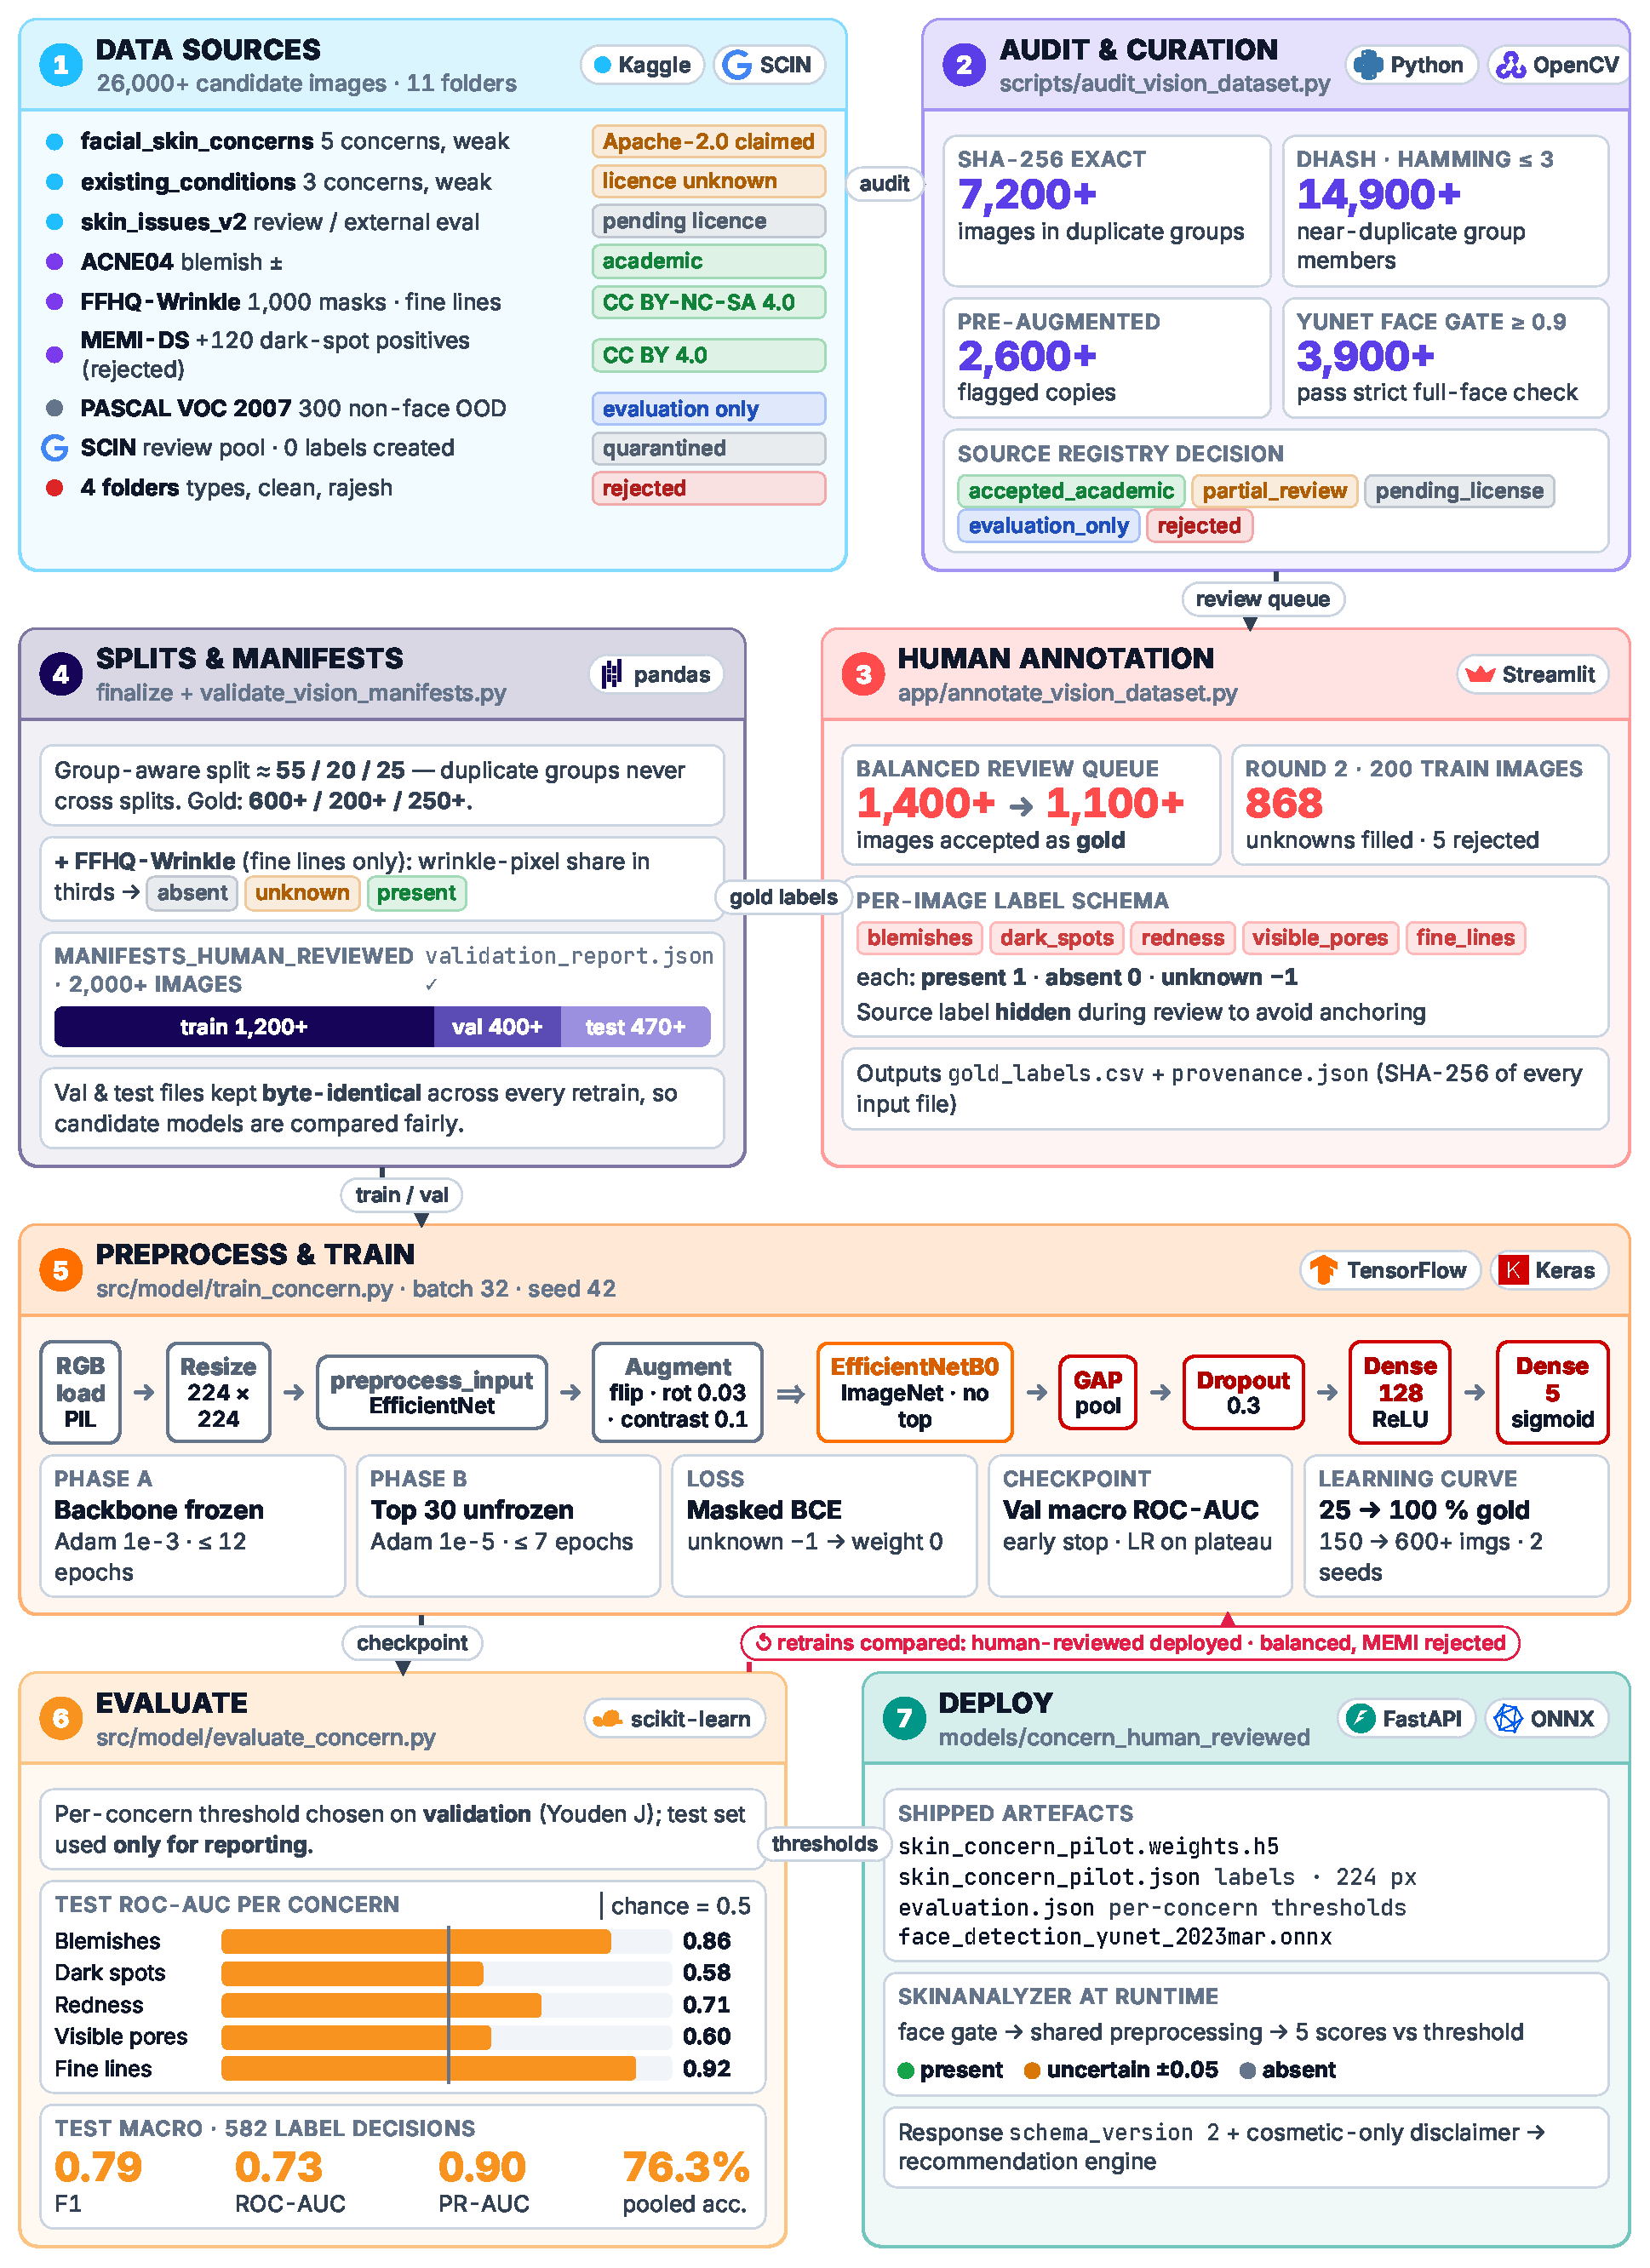
\includegraphics[width=\linewidth]{figures/pipeline.pdf}
\caption{Data and model development pipeline}
\label{fig:pipeline}
\end{figure}

\subsubsection*{Methods for each objective}

Table~\ref{tab:methods} summarises the method, tools and evidence for each objective. The key method details follow the table.

\begin{table}[ht]
\centering\small
\caption{Methods, tools and evidence for each objective}
\label{tab:methods}
\begin{tabularx}{\linewidth}{P{1.9cm}P{3.6cm}P{3.1cm}Y}
\toprule
\textbf{Objective} & \textbf{Method} & \textbf{Main tools} & \textbf{Output and evidence}\\
\midrule
O1 Dataset & Data audit, human annotation, group-aware splitting & SHA-256, dHash, YuNet, Streamlit & Source registry, annotation files, validated manifests\\
O2 Model & Supervised transfer learning, multi-label with masked loss & TensorFlow/Keras, EfficientNetB0 & Weights, \texttt{evaluation.json} with weight hash\\
O3 Catalogue & Web scraping and data cleaning & Python, pandas, rapidfuzz & Unified product CSV\\
O4 Recommender & Rule-based content filtering with a weighted score & Python & Ranked products with matched ingredients\\
O5 Application & Client--server development & FastAPI, Expo/React Native & Running app, API contract tests\\
O6 Evaluation & Mixed methods: metrics, functional tests, heuristic review, survey & unittest, curl, Google Forms & Evidence files, test tables, survey responses\\
\bottomrule
\end{tabularx}
\end{table}

\textbf{Data audit and annotation (O1).} Every candidate image was hashed twice. SHA-256 found exact copies, and a 64-bit difference hash (dHash) with a Hamming radius of 3 found near-duplicates. A YuNet face detector \citep{wu2023yunet} recorded whether each image showed a full face, a close-up or no face. Each source was entered in a registry with its licence, provenance and decision.

Images were then labelled in a purpose-built Streamlit tool, following a written guide (Appendix~\ref{app:annotation}). Each concern was marked \emph{present}, \emph{absent} or \emph{unknown}, and the original folder label was hidden to reduce anchoring bias. A first queue of 1,400+ images was reviewed, followed by a second review of 200 training images whose labels were still unknown. FFHQ-Wrinkle masks \citep{moon2024} were converted to fine-line labels by wrinkle-pixel coverage: the lowest third became absent, the highest third present, and the middle third unknown.

Duplicate groups were assigned to a split as a unit, at roughly 55/20/25. No near-duplicate can therefore appear in both training and testing \citep{barz2020,kapoor2023}.

\textbf{Model training (O2).} The model is an ImageNet-pretrained EfficientNetB0 \citep{tan2019} with a five-output sigmoid head. It is trained with \emph{masked} binary cross-entropy, so unknown labels contribute no gradient and ``not annotated'' is never treated as ``absent'' \citep{liu2022multilabel}. Training has two phases: the head is trained with the backbone frozen (Adam, learning rate $10^{-3}$), then the top 30 layers are fine-tuned (learning rate $10^{-5}$). The final checkpoint is chosen on validation data only.

Each concern's threshold maximises Youden's $J$ (bookmaker informedness) on validation data \citep{chicco2021}. The test set is used only for reporting. Because positives dominate most concerns, balanced accuracy and ROC-AUC are reported next to F1, which on its own rewards always predicting ``present'' \citep{chicco2020}.

\textbf{Catalogue and recommender (O3, O4).} Product pages from Jeevee, ForEveryNG and Oriflame were scraped to CSV and normalised to one schema. Near-duplicate products were merged using \texttt{rapidfuzz} token-sort similarity ($\geq 85$), keeping the most complete record. Category, ingredient and skin-type tags were inferred from keyword dictionaries. Each concern maps to beneficial ingredients and categories (Table~\ref{tab:rules}), and products are ranked by a weighted linear score (Section~\ref{sec:recommender}).

\textbf{Application (O5).} A FastAPI REST backend wraps the model, face gate, recommender and language model. An Expo (React Native) client provides the interface. The two communicate only through a versioned JSON contract that is covered by a unit test.

\subsubsection*{Evaluation design (O6)}

The evaluation has five strands, chosen so that each one covers a weakness of the others:
\begin{enumerate}
  \item \textbf{Held-out model metrics} for every model version, on the same fixed test set.
  \item \textbf{A learning-curve study}, retraining on 25--100\% of the data, to test whether more data would help.
  \item \textbf{Black-box functional tests}: 19 documented cases run against the live API.
  \item \textbf{A heuristic evaluation} of the running app against Nielsen's ten heuristics \citep{galavi2024}.
  \item \textbf{A participant usability survey.} Participants install and use the app, complete four set tasks (check a photo, read the result, find a product, ask the assistant), then answer a Google Form. The form contains consent, anonymous background questions, task completion and ease ratings, the ten-item System Usability Scale \citep{vlachogianni2022}, and questions about trust and understanding of the results. No names, emails or photos are collected. The full protocol is in Appendix~\ref{app:usability}.
\end{enumerate}

\subsection{Justification of Methods}

\textbf{Iterative process and CRISP-DM rather than a fixed plan.} The data's quality was unknown at the start. A fixed, waterfall-style plan would have committed the project to the disease classifier before the audit showed it was unsafe. An iterative process made it possible to change direction on evidence \citep{schroer2021}.

\textbf{Transfer learning rather than training from scratch.} With only 1,200+ training images, a CNN trained from scratch would overfit badly. ImageNet features give a strong starting point for texture and colour \citep{zhuang2021}. EfficientNetB0 was chosen over the planned B2 because it has about 5.3 million parameters, compared with about 9.2 million for B2. On a CPU-only backend, the smaller model's speed outweighed any small accuracy gain that B2 might have given.

\textbf{Multi-label with masking rather than multi-class.} Concerns co-occur on real faces, so a single softmax label would force the model to pick one. Masking lets partially labelled images still contribute: an image labelled only for fine lines still trains the fine-lines output.

\textbf{Audit and human review rather than accepting folder labels.} The folder labels in the Kaggle sources were contaminated (Section~\ref{sec:construction}). Training on them would have produced impressive but meaningless accuracy. Human review is slower, but it is the only way to obtain labels whose meaning is defined.

\textbf{Skin type from the user rather than from the photo.} The only skin-type image source was rejected (100+ images, including stock photographs). Oiliness and dryness are also partly tactile, so they are hard to judge from one photo. Asking the user is more reliable and more respectful.

\textbf{Weighted rules rather than TF-IDF similarity or collaborative filtering.} Collaborative filtering needs interaction histories that do not exist \citep{ricci2022}. TF-IDF over ingredient text was planned, but scraped listings rarely include full ingredient lists: 65\% of products have no inferable ingredient at all. A weighted score over explicit features is simpler, degrades predictably and can be explained line by line \citep{roy2022}.

\textbf{Grounded language model rather than free generation.} Qwen2.5 \citep{qwen2024} runs locally without a paid API. Its outputs are restricted in code, not only by the prompt, to product IDs in the candidate set. It is optional, and the core flow never depends on it. This limits the hallucination risk \citep{ji2023}.

\textbf{Heuristic review and an online survey together.} A heuristic review finds many interface problems cheaply, but it reflects only the evaluator's view \citep{galavi2024}. A survey with SUS captures how real users perceive the app and gives a score that can be compared with published benchmarks \citep{vlachogianni2022}. Google Forms was chosen because it is free, needs no account for participants, records responses anonymously, and exports directly to CSV for analysis.

\section{Artefact Design}
\label{sec:artefact}

This section gives a factual description of the artefact as built: its requirements (Table~\ref{tab:spec}) and its architecture (Figure~\ref{fig:arch}).

\subsection{Design Specifications}

\begin{table}[ht]
\centering\small
\caption{Design specification: functional (F) and non-functional (N) requirements}
\label{tab:spec}
\begin{tabularx}{\linewidth}{lYl}
\toprule
\textbf{ID} & \textbf{Requirement} & \textbf{Obj.}\\
\midrule
F1 & Accept a JPEG/PNG face photo up to 10\,MB from camera or gallery & O5\\
F2 & Reject images without a detectable face and explain how to retake the photo & O5\\
F3 & Return a score, threshold and status (\emph{present}, \emph{absent} or \emph{uncertain}) for each of five concerns & O2\\
F4 & Accept an optional user skin type (dry, normal, oily, combination, sensitive); never infer it from the photo & O4\\
F5 & Recommend up to five products per relevant category, with the matched ingredients and a score & O4\\
F6 & Suggest a morning and evening routine derived from the detected concerns & O4\\
F7 & Browse, search, filter and sort the catalogue; view product detail; save favourites & O5\\
F8 & Keep a local history of past checks & O5\\
F9 & Answer free-text questions through a grounded chat assistant, falling back to rules if the language model is unavailable & O5\\
F10 & Show a non-medical disclaimer on every result and chat screen & O5\\
\midrule
N1 & No medical labels; wording must describe observations, not diagnoses & --\\
N2 & Thresholds are set on validation data only; the test set is used only for reporting & O2\\
N3 & Photos are not stored on the server; history is kept on the device only & --\\
N4 & Warm analysis completes in under 2 seconds on a laptop CPU & O5\\
N5 & Runs entirely on free, open-source software without paid APIs & --\\
N6 & Structured API errors (400/404/422/500) so the client can show helpful messages & O5\\
\bottomrule
\end{tabularx}
\end{table}

\subsection{Artefact's Structure/ Architecture / Framework}

\subsubsection*{Architectural style}

SkinCare AI uses a \textbf{three-tier client--server architecture} (Figure~\ref{fig:arch}):
\begin{enumerate}
  \item a \emph{presentation tier}, the Expo/React Native mobile client;
  \item an \emph{application tier}, a stateless FastAPI REST service that holds the model, face gate, recommender and language model in memory;
  \item a \emph{data tier} of read-only files: model weights and thresholds, the product catalogue and the ingredient mappings.
\end{enumerate}

Three design principles shape this structure:
\begin{itemize}
  \item \textbf{Separation of concerns.} The client only collects input and displays results. All analysis and ranking happens on the server, so the model can be replaced without changing the app.
  \item \textbf{Statelessness and privacy by design.} The server stores no photos and no user data. Each request carries everything needed to answer it, and history and favourites are kept only on the device (requirement N3).
  \item \textbf{Graceful degradation.} The language model is optional. If it is unavailable, slow or returns invalid output, a deterministic rule-based answer is used, so the core photo-to-product flow never depends on it.
\end{itemize}

\begin{figure}[p]
\centering
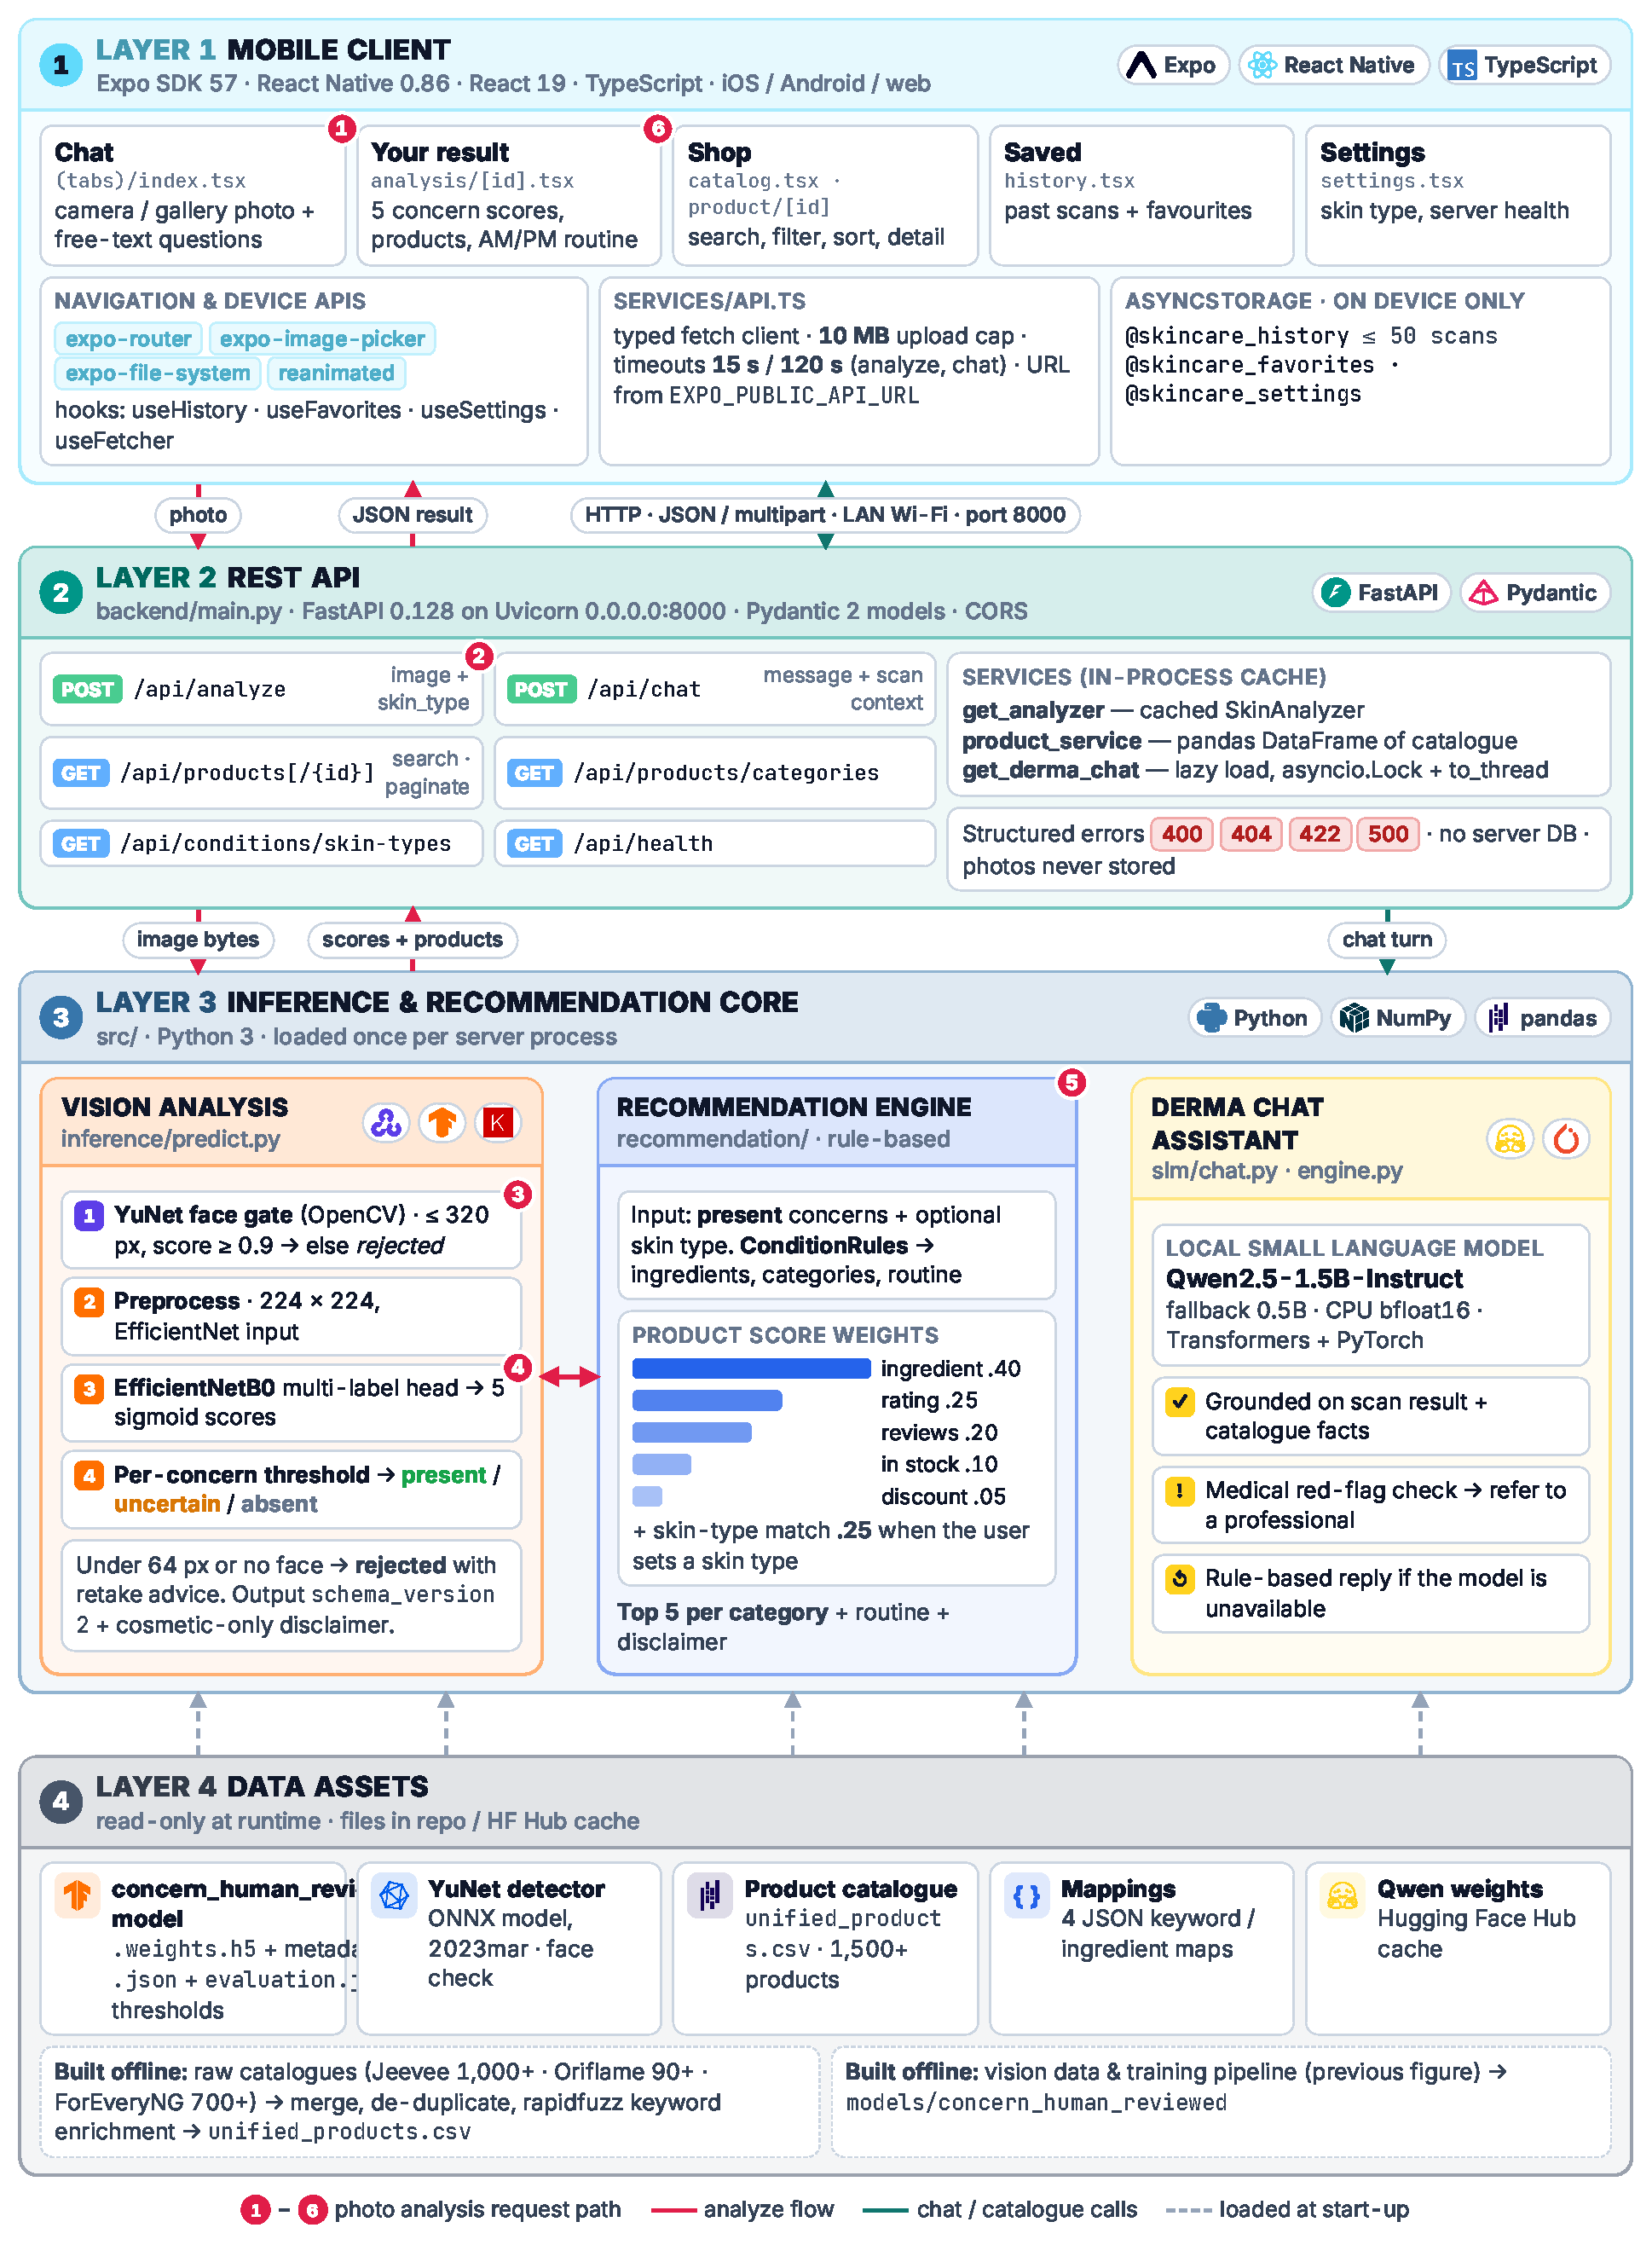
\includegraphics[width=\linewidth]{figures/architecture.pdf}
\caption{System architecture of SkinCare AI: Expo/React Native client, FastAPI layer, Python inference and recommendation core (TensorFlow, OpenCV, Transformers), and data assets}
\label{fig:arch}
\end{figure}

\subsubsection*{Components}

Table~\ref{tab:components} lists the main components, what each is responsible for and where it lives in the code.

\begin{table}[ht]
\centering\small
\caption{Main components of the artefact}
\label{tab:components}
\begin{tabularx}{\linewidth}{P{2.6cm}YP{4.3cm}}
\toprule
\textbf{Component} & \textbf{Responsibility} & \textbf{Implementation}\\
\midrule
Mobile client & Tabs for Chat, Shop, Saved and Settings; photo capture; result, routine and product screens; on-device history and favourites & \texttt{mobile/app}, \texttt{mobile/services/api.ts}, AsyncStorage hooks\\
API layer & Validates uploads and parameters, routes requests, returns structured errors (400/404/422/500) & FastAPI routers in \texttt{backend/routes}\\
Face gate & Rejects photos without a clear face (YuNet score $\geq 0.9$) & \texttt{SkinAnalyzer} with OpenCV \texttt{FaceDetectorYN}\\
Concern model & Shared preprocessing, five sigmoid scores, per-concern thresholds and status & \texttt{SkinAnalyzer} in \texttt{predict.py}; shared \texttt{concern\_\allowbreak preprocessing.py}\\
Recommender & Maps present concerns to ingredients and categories; ranks products by weighted score & \texttt{RecommendationEngine}, \texttt{ConditionRules}, \texttt{scoring.py}\\
Language-model layer & Optional re-ranking and grounded chat; rule-based fallback; red-flag signposting & \texttt{SlmEngine}, \texttt{DermaChat}, \texttt{SlmRecommender} (Qwen2.5)\\
Data assets & Model weights, \texttt{evaluation.json} thresholds, product catalogue, ingredient mappings & \texttt{models/}, \texttt{data/enriched}, \texttt{data/mappings}\\
\bottomrule
\end{tabularx}
\end{table}

\subsubsection*{API interface}

The client and server communicate only through the REST endpoints in Table~\ref{tab:api}. Analysis responses carry a schema version, the model version and the disclaimer, and their structure is fixed by a contract unit test.

\begin{table}[ht]
\centering\small
\caption{REST API endpoints}
\label{tab:api}
\begin{tabularx}{\linewidth}{lP{4.9cm}Y}
\toprule
\textbf{Method} & \textbf{Path} & \textbf{Purpose}\\
\midrule
GET & \texttt{/api/health} & Connection check used by the app's ``Test connection'' button\\
POST & \texttt{/api/analyze} & Multipart photo plus optional skin type; returns concerns, routine and recommendations\\
POST & \texttt{/api/chat} & Question plus optional latest result; returns a grounded reply and product cards\\
GET & \texttt{/api/products} & Catalogue search, filter by category and skin type, sort and paginate\\
GET & \texttt{/api/products/categories} & List of product categories\\
GET & \texttt{/api/products/\{id\}} & Product detail, or 404\\
GET & \texttt{/api/conditions/skin-types} & The five skin types with recommended ingredients\\
\bottomrule
\end{tabularx}
\end{table}

\subsubsection*{Analysis request flow}

When the client uploads a photo to \texttt{/api/analyze}, the server processes it in five steps:
\begin{enumerate}
  \item It checks the MIME type and size of the upload.
  \item It decodes the image to RGB and runs YuNet on a copy resized to at most 320\,px. If no face scores at least 0.9, it returns a \emph{rejected} result that explains how to retake the photo.
  \item It preprocesses the image exactly as during training: bilinear resize to 224$\times$224 followed by EfficientNet normalisation. This code is shared by training, evaluation and serving.
  \item It predicts five sigmoid scores. A score within $\pm0.05$ of its concern's threshold is labelled \emph{uncertain}, a higher score \emph{present}, and a lower score \emph{absent}.
  \item It passes the concerns marked \emph{present}, and the stated skin type, to the recommender, and returns the combined result.
\end{enumerate}

\subsubsection*{Core modules}

\textbf{Model.} The network is EfficientNetB0 without its ImageNet head, followed by global average pooling, dropout (0.3), a 128-unit ReLU layer and a 5-unit sigmoid output. It has about 4.2 million parameters in total. Per-concern thresholds are loaded from the model's \texttt{evaluation.json} file, so re-evaluating the model updates the live app without any code change.

\label{sec:recommender}
\textbf{Recommender.} Table~\ref{tab:rules} lists the rule map. For each category relevant to the present concerns, every product in that category receives a score:
\begin{equation}
s = w_i\,I + w_r\,\tfrac{\text{rating}}{5} + w_v\,\tfrac{\log(1+\text{reviews})}{\log 1001} + w_a\,\mathbf{1}[\text{in stock}] + w_d\,\min(2\cdot\text{discount},1) + w_t\,T
\end{equation}
Here $I$ is the fraction of target ingredients that the product contains, and $T$ is its match to the stated skin type. The weights are $(w_i,w_r,w_v,w_a,w_d,w_t) = (0.40,0.25,0.20,0.10,0.05,0)$ when no skin type is given, and $(0.35,0.20,0.12,0.06,0.02,0.25)$ when one is. The top five products per category are returned together with the ingredients they matched. If no concern is present, a basic cleanser, moisturiser and sunscreen routine is suggested.

\begin{table}[ht]
\centering\small
\caption{Concern-to-ingredient and category rules used by the recommender}
\label{tab:rules}
\begin{tabularx}{\linewidth}{lYY}
\toprule
\textbf{Concern} & \textbf{Target ingredients} & \textbf{Categories}\\
\midrule
Blemishes & salicylic acid, niacinamide, tea tree, zinc, glycolic acid & cleanser, serum, moisturiser, spot treatment, toner\\
Dark spots & vitamin C, niacinamide, kojic acid, arbutin, glycolic acid, azelaic acid & cleanser, serum, moisturiser, spot treatment, sunscreen\\
Redness & centella asiatica, ceramides, aloe vera, niacinamide, panthenol & cleanser, moisturiser, sunscreen, serum\\
Visible pores & niacinamide, salicylic acid, zinc, glycolic acid & cleanser, toner, serum, moisturiser\\
Fine lines & retinol, hyaluronic acid, peptides, ceramides, vitamin C & cleanser, serum, moisturiser, sunscreen\\
\bottomrule
\end{tabularx}
\end{table}

\textbf{Language-model layer.} \texttt{Qwen2.5-1.5B-Instruct}, with a \texttt{0.5B} fallback, runs on the CPU. It is used in two places:
\begin{itemize}
  \item optionally, to reorder and justify the top candidates in an analysis result;
  \item for the chat assistant.
\end{itemize}
The prompt contains only catalogue facts for the candidate products. The response is parsed as JSON, and any product ID not in the candidate list is discarded in code. If the model is unavailable, or produces nothing valid, a deterministic rule-based answer is returned instead.

\textbf{Technology stack.} Table~\ref{tab:stack} summarises the stack.

\begin{table}[ht]
\centering\small
\caption{Technology stack}
\label{tab:stack}
\begin{tabularx}{\linewidth}{lY}
\toprule
\textbf{Layer} & \textbf{Technologies}\\
\midrule
Model \& data & Python 3.9, TensorFlow 2.16 / Keras, OpenCV (YuNet), pandas, NumPy, rapidfuzz, Pillow\\
Backend & FastAPI, Uvicorn, Pydantic, Hugging Face Transformers (Qwen2.5)\\
Mobile & Expo SDK, React Native, expo-router, TypeScript, AsyncStorage, expo-image-picker\\
Tooling & Streamlit (annotation and demonstration), Git, unittest\\
\bottomrule
\end{tabularx}
\end{table}

\section{Implementation}
\label{sec:impl}

This section describes how the artefact was built (Section~\ref{sec:construction}) and how it was validated (Section~\ref{sec:validation}). It links each step to the problem statement: producing trustworthy, locally actionable skincare guidance.

\subsection{Construction of the Artefact}
\label{sec:construction}

\subsubsection*{Iteration 1: disease and skin-type prototype (August 2026)}

The first version followed the interim plan. Images from several Kaggle collections were merged into folders for seven conditions (including carcinoma) and three skin types. A multi-task EfficientNetB0 was trained on these folders. The Streamlit and mobile interfaces showed the predicted condition, and a carcinoma prediction triggered a ``see a dermatologist'' message.

This iteration proved that the full pipeline could be integrated, from photo to API to recommendations. However, as the progress review recorded, it produced no trustworthy metrics. Manual trials also suggested poor real-world accuracy.

\subsubsection*{Iteration 2: data audit (September 2026)}

Rather than tune the model further, the data was audited. This proved to be the most important decision in the project. Table~\ref{tab:audit} summarises the findings across more than 26,000 files drawn from the original folders and four additional candidate collections.

\begin{table}[ht]
\centering\small
\caption{Findings of the vision data audit}
\label{tab:audit}
\begin{tabular}{lr}
\toprule
\textbf{Finding} & \textbf{Count}\\
\midrule
Files audited & 26,000+\\
Pre-generated (already augmented) images & 2,600+\\
Exact-duplicate groups / images involved & 3,200+ / 7,200+\\
Perceptual-duplicate groups / images involved & 5,200+ / 14,900+\\
Perceptual groups spanning different sources & 2,400+\\
Images passing the strict full-face gate & 3,900+\\
\bottomrule
\end{tabular}
\end{table}

More than half of all images belonged to a perceptual-duplicate group. Thousands of duplicates crossed source boundaries, which shows that the Kaggle collections had re-uploaded each other. The ``cleaned'' train/validation split that came with the original data contained repeated stock images and augmentations, so it leaked into its own validation set. Any accuracy measured on it would have been inflated \citep{barz2020}.

The skin-type folder held only 100+ images, including stock photographs whose labels could not be verified. The condition folders mixed medical diagnoses with cosmetic appearance and had no provenance.

These findings led to three decisions:
\begin{enumerate}
  \item drop disease labels, and with them any implied medical claim;
  \item stop predicting skin type from photographs and ask the user instead;
  \item redefine the task as five visible cosmetic concerns, labelled by a human against written definitions.
\end{enumerate}
The source registry (Table~\ref{tab:sources}) records the outcome for every source.

\begin{table}[ht]
\centering\small
\caption{Source registry decisions}
\label{tab:sources}
\begin{tabularx}{\linewidth}{lllY}
\toprule
\textbf{Source} & \textbf{Images} & \textbf{Decision} & \textbf{Reason}\\
\midrule
Original condition folders & 7,600+ & Partial & Only acne, dark-spot and rosacea folders reviewed; no provenance\\
Kaggle facial skin concerns & 4,200+ & Partial & Useful coverage; watermarks and label noise\\
Kaggle skin issues v2 & 9,700+ & Pending & Unknown licence; heavy overlap\\
Original ``cleaned'' split & 3,200+ & Rejected & Stock images, augmentations, leakage\\
Kaggle normal/oily/dry & 1,400+ & Rejected & Stock images, invalid skin-type labels\\
Original skin-type folder & 100+ & Rejected & Too small; photo-based skin type out of scope\\
ACNE04 \citep{wu2019acne} & 390+ & Accepted & Academic dataset, known provenance\\
FFHQ-Wrinkle \citep{moon2024} & 1,000 & Accepted & Manual wrinkle masks, CC BY-NC-SA\\
SCIN \citep{ward2024} & 70 & Quarantined & 0 of 70 passed the full-face gate; no cosmetic labels\\
PASCAL VOC 2007 \citep{everingham2010} & 300 & Test only & Non-face images for face-gate testing\\
\bottomrule
\end{tabularx}
\end{table}

\subsubsection*{Iteration 3: annotation, training and deployment}

A review queue of 1,400+ images, balanced by source and concern, was labelled in a custom Streamlit annotator. Of these, 1,100+ images were accepted and the rest were rejected as unusable. Most labels remained \emph{unknown}, which is the honest answer for close-ups showing one region.

Negative examples were very scarce. In the first gold set, fewer than 20 images were labelled as having no blemishes, and fewer than 35 as having no redness. Fine lines had the most balanced labels, so FFHQ-Wrinkle was added to strengthen that concern.

The first manifests contained 2,000+ images. Training used seed 42, horizontal-flip, rotation and contrast augmentation, and the two-phase schedule described in Section~\ref{sec:design}. Training refuses to overwrite existing weights, so every run is preserved. This model (\texttt{concern\_v2}) was deployed first, and its weak results for blemishes, redness and pores (Section~\ref{sec:validation}) were traced to the very small number of negative training labels: only 9 for blemishes and 19 each for redness and pores.

Two further engineering problems were found and fixed during this iteration.

\begin{itemize}
  \item \textbf{Train/serve preprocessing mismatch.} The backend originally resized images with a different method from the one used in training. Moving preprocessing into one shared module raised the pooled label accuracy of \texttt{concern\_v2} on the test set from 70.3\% to 73.2\% with no retraining. This shows how silent inconsistencies can erode deployed performance.
  \item \textbf{Degenerate thresholds.} Choosing thresholds by maximising F1 on validation data set the dark-spot and pore thresholds to 0.0, so those concerns were \emph{always} reported as present. Switching to Youden's $J$, which rewards specificity as well as recall, produced meaningful thresholds (Table~\ref{tab:results}).
\end{itemize}

\subsubsection*{Iteration 4: second label review and retraining}

Two attempts were made to fix the shortage of negative examples.
\begin{itemize}
  \item \textbf{Class reweighting} gave each concern's positive and negative labels equal total weight. It did not help on the test set and was rejected (Table~\ref{tab:modelcompare}).
  \item \textbf{A second human review} targeted the 200 training images whose dark-spot, redness or pore labels were still unknown. Every image was re-examined against the same guide. The merge filled 868 previously unknown labels and removed five images judged unusable. Seven disagreements with existing fine-line labels were logged and the original labels were kept. Validation and test files were copied unchanged and verified by hash.
\end{itemize}

The second review raised the number of negative training labels sharply: from 9 to 159 for blemishes, from 19 to 188 for redness, and from 19 to 71 for visible pores (Table~\ref{tab:splits}). The model was then fine-tuned from the \texttt{concern\_v2} weights with the same seed and no class reweighting. The best checkpoint on validation macro ROC-AUC was selected (0.706, compared with 0.686 for \texttt{concern\_v2}). Its thresholds were again chosen on validation data only. This model, \texttt{concern\_human\_reviewed}, scored higher than \texttt{concern\_v2} on all four macro test metrics and is now the deployed model.

A final experiment added 120+ melasma photographs from the MEMI dataset to the training split as extra dark-spot positives. It did not improve dark spots and lowered overall accuracy, so it was not deployed.

\begin{table}[ht]
\centering\small
\caption{Data splits of the deployed model (positive/negative known labels; unknown labels are excluded from the loss)}
\label{tab:splits}
\begin{tabular}{lrrrrrr}
\toprule
\textbf{Split} & \textbf{Images} & \textbf{Blemishes} & \textbf{Dark spots} & \textbf{Redness} & \textbf{Pores} & \textbf{Fine lines}\\
\midrule
Train & 1,200+ & 274/159 & 204/188 & 249/188 & 228/71 & 362/390\\
Validation & 400+ & 68/4 & 36/22 & 64/6 & 33/11 & 123/95\\
Test & 470+ & 97/4 & 65/22 & 97/8 & 46/9 & 116/118\\
\bottomrule
\end{tabular}
\end{table}

\subsubsection*{Catalogue and recommender}

Scraping produced 700+ ForEveryNG, 1,000+ Jeevee and 90+ Oriflame rows. After normalisation and fuzzy deduplication, 1,500+ unique products remained: 800+ from Jeevee, 600+ from ForEveryNG and 70+ from Oriflame. They cover 650+ brands, with a median price of Rs.~799, and 99\% of them are in stock.

Keyword inference assigned a category to 82\% of products. However, it found at least one target ingredient for only 35\% of products (500+), and a skin-type tag for 38\%, because most listings name only headline actives. This limits the ingredient component of the score (Section~\ref{sec:eval}).

\subsubsection*{Mobile application}

The Expo client has four tabs: Chat, Shop, Saved and Settings. Photos are added from the chat screen (the ``+'' button), which keeps analysis and follow-up questions in one conversation. Results open a detail screen with the following elements:
\begin{itemize}
  \item score bars with a threshold tick;
  \item the status of each concern;
  \item a morning and evening routine;
  \item recommendations grouped by category, with ``Fits'' ingredient tags.
\end{itemize}
The server address is discovered automatically on the local network, and structured API errors are translated into plain-language messages. Figure~\ref{fig:screens} shows screenshots captured from the running application.

\textbf{User journey.} A first-time user opens the app on the Chat tab, where an empty-state prompt invites them to tap ``+'' to check a photo or to type a question. Before any analysis, the user can set a skin type in Settings; the screen states that skin type is ``never guessed from photos'', and it may be left unset. Tapping ``+'' offers the camera or the gallery, with an instruction to use ``one clear, front-facing photo of your whole face in daylight''. The result appears as a card that opens the detail screen. Tapping a product opens its detail page, where it can be saved to the user's ``shelf''. Every result is stored in the on-device history under the Saved tab, and the assistant receives the latest result as context, so follow-up questions can refer to the user's own concerns and recommended products.

\begin{figure}[p]
\centering
\begin{subfigure}[t]{0.24\linewidth}
\includegraphics[width=\linewidth]{figures/chat.png}\caption{Grounded chat}\end{subfigure}\hfill
\begin{subfigure}[t]{0.24\linewidth}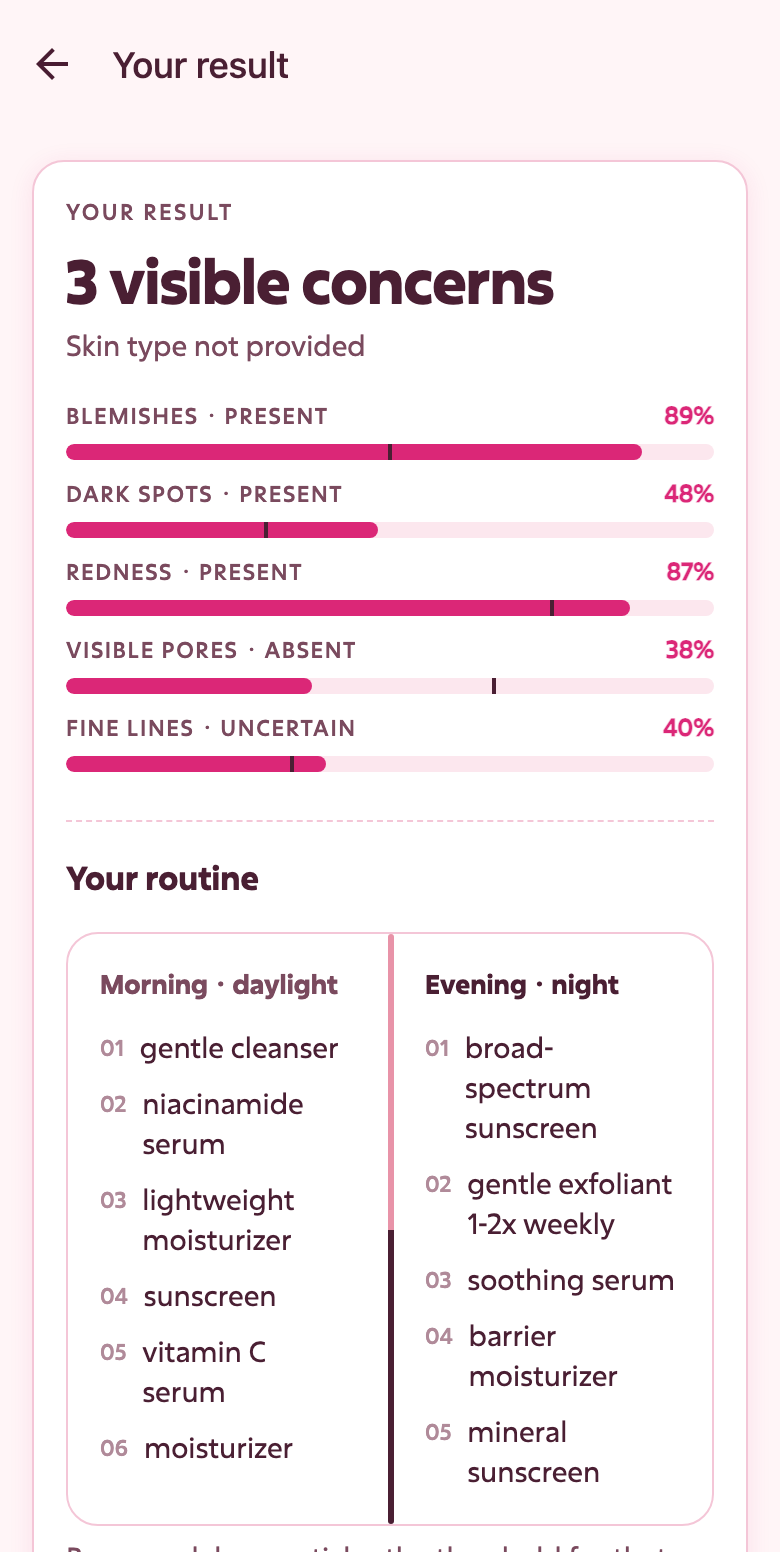
\includegraphics[width=\linewidth]{figures/analysis.png}\caption{Concern result}\end{subfigure}\hfill
\begin{subfigure}[t]{0.24\linewidth}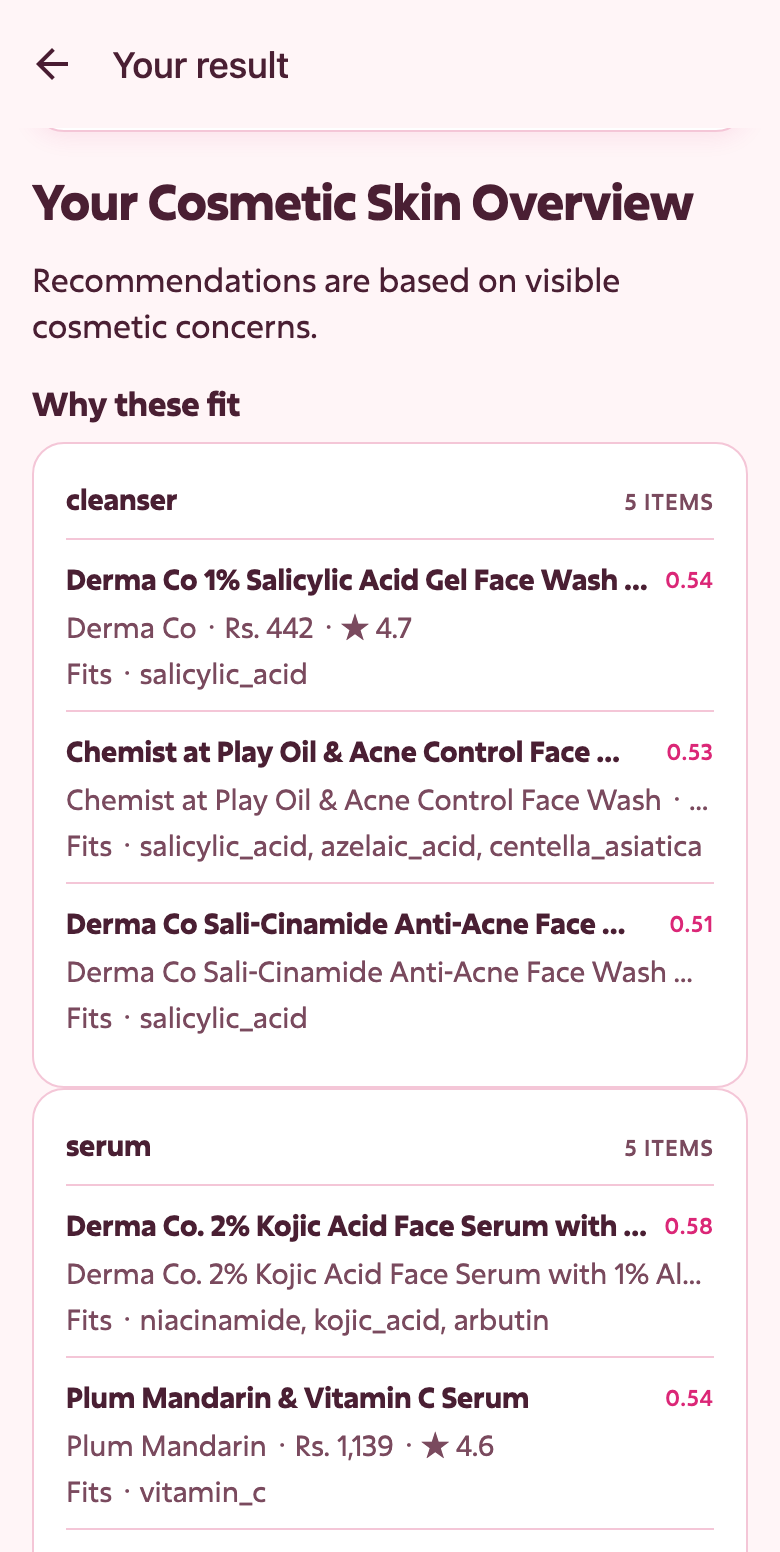
\includegraphics[width=\linewidth]{figures/analysis_1.png}\caption{Recommendations}\end{subfigure}\hfill
\begin{subfigure}[t]{0.24\linewidth}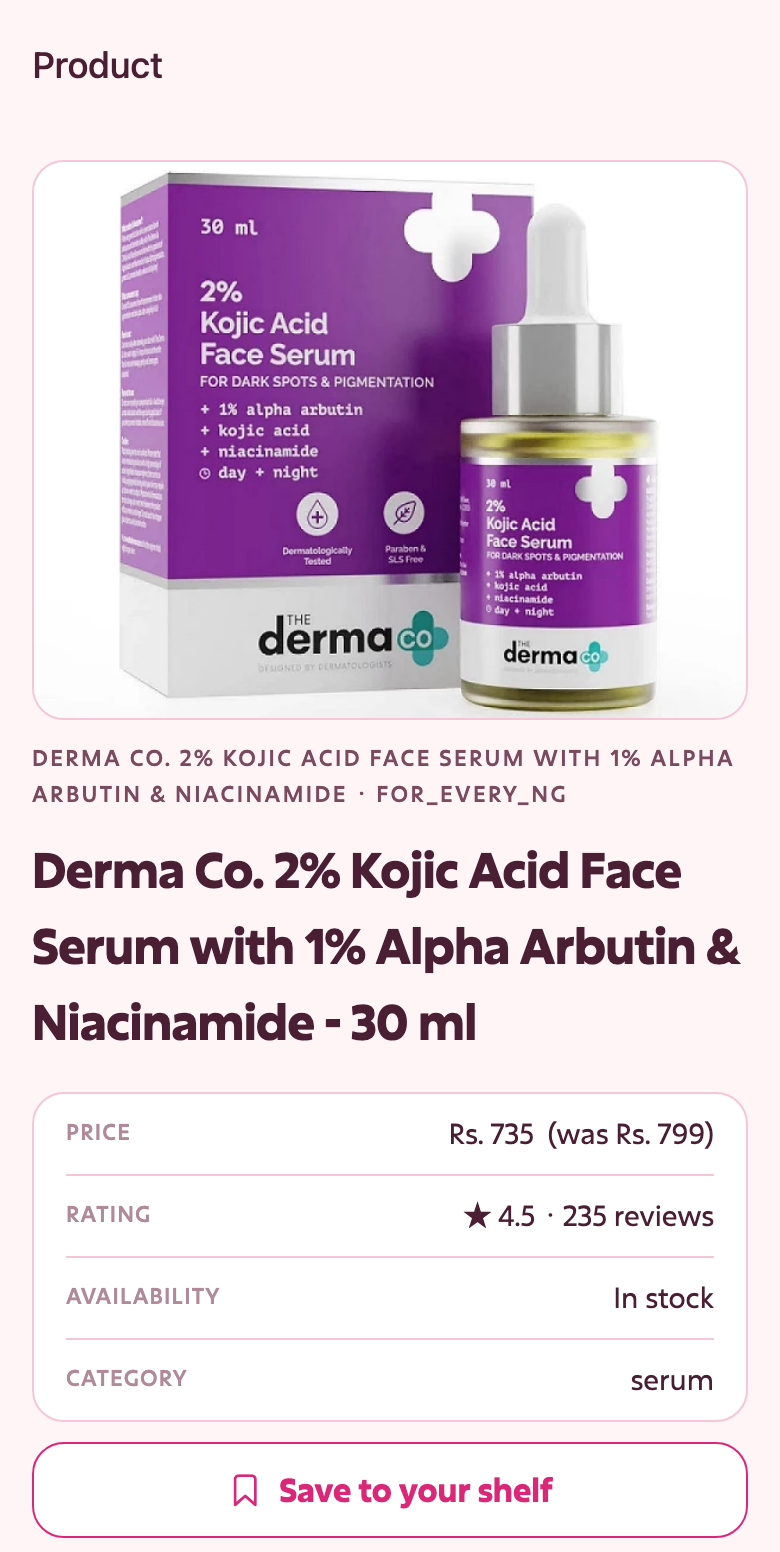
\includegraphics[width=\linewidth]{figures/product.png}\caption{Product detail}\end{subfigure}\\[8bp]
\begin{subfigure}[t]{0.24\linewidth}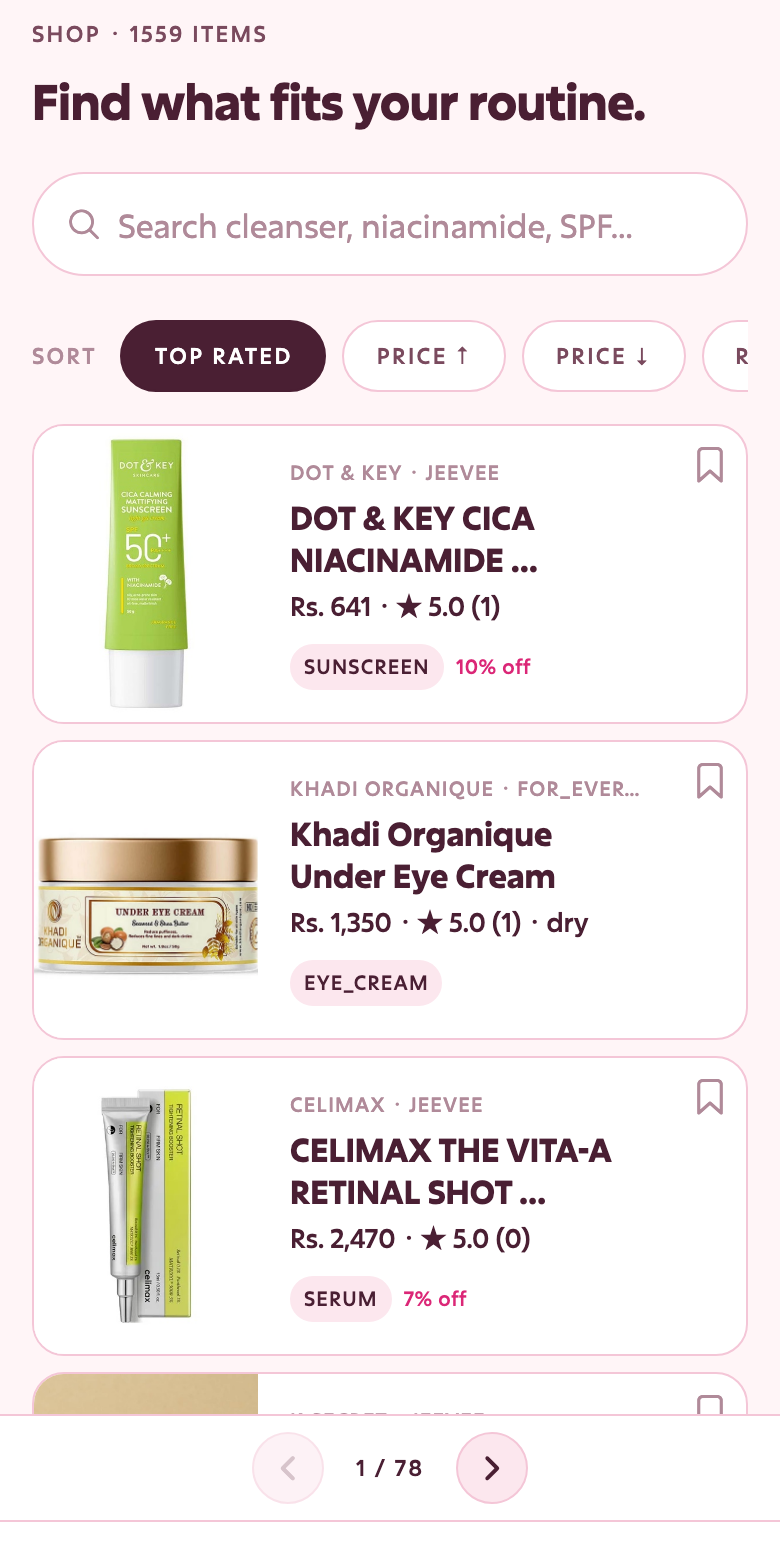
\includegraphics[width=\linewidth]{figures/catalog.png}\caption{Catalogue}\end{subfigure}\hfill
\begin{subfigure}[t]{0.24\linewidth}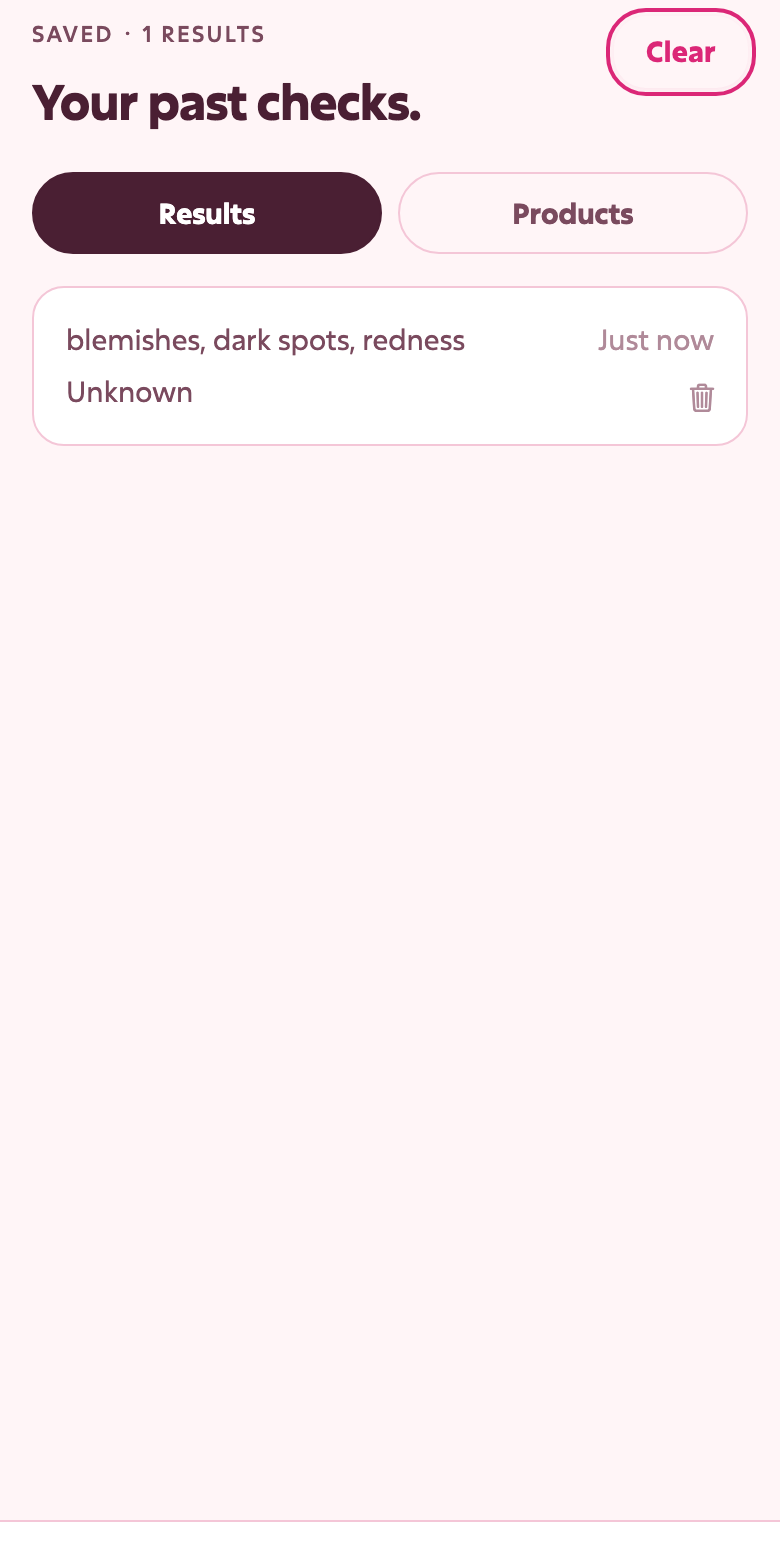
\includegraphics[width=\linewidth]{figures/history.png}\caption{History}\end{subfigure}\hfill
\begin{subfigure}[t]{0.24\linewidth}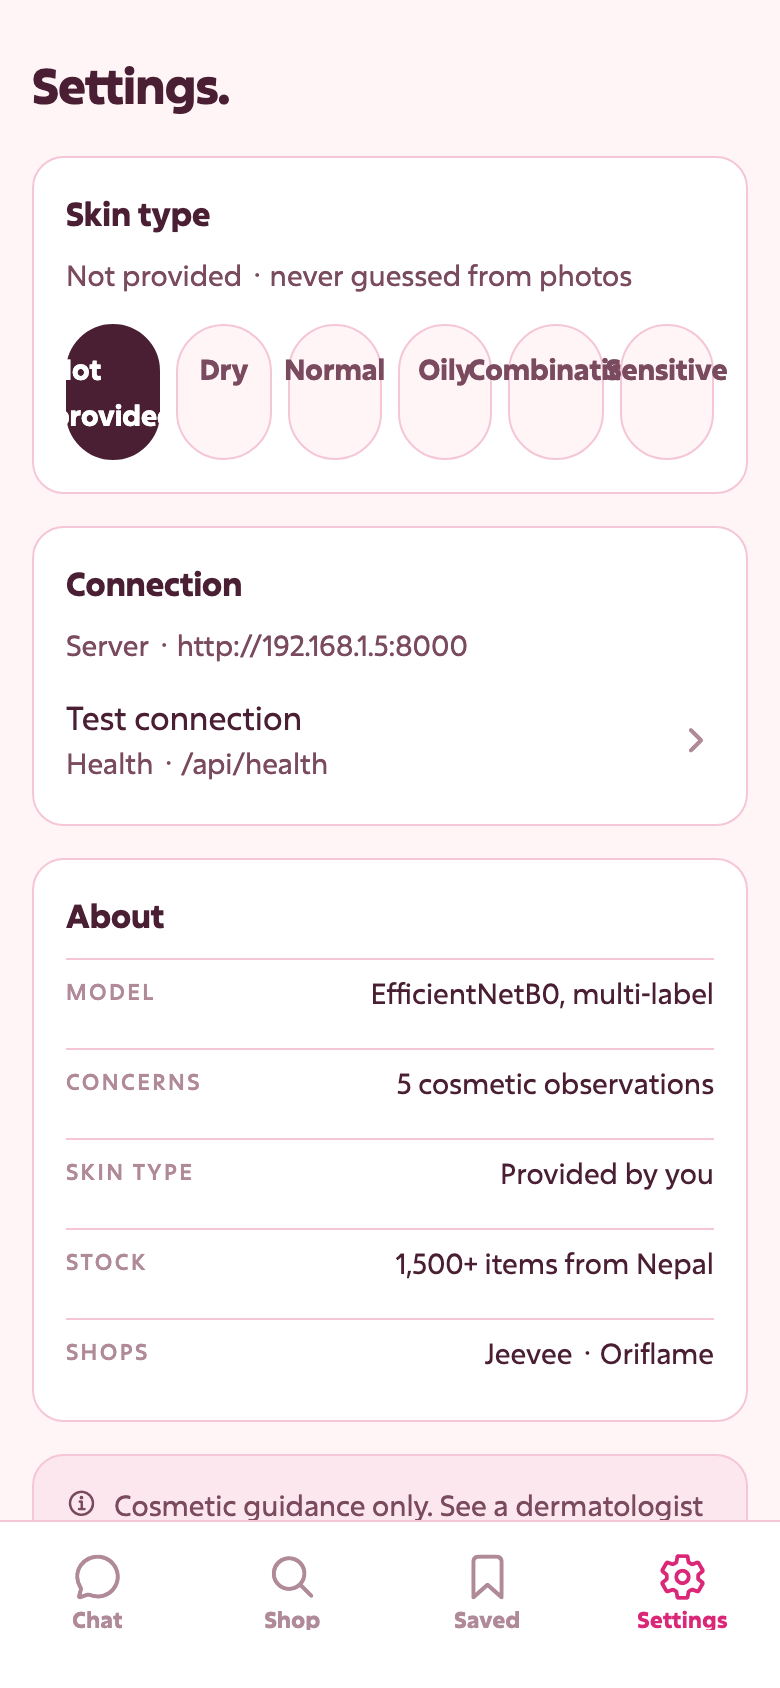
\includegraphics[width=\linewidth]{figures/settings.png}\caption{Settings}\end{subfigure}\hfill
\begin{subfigure}[t]{0.24\linewidth}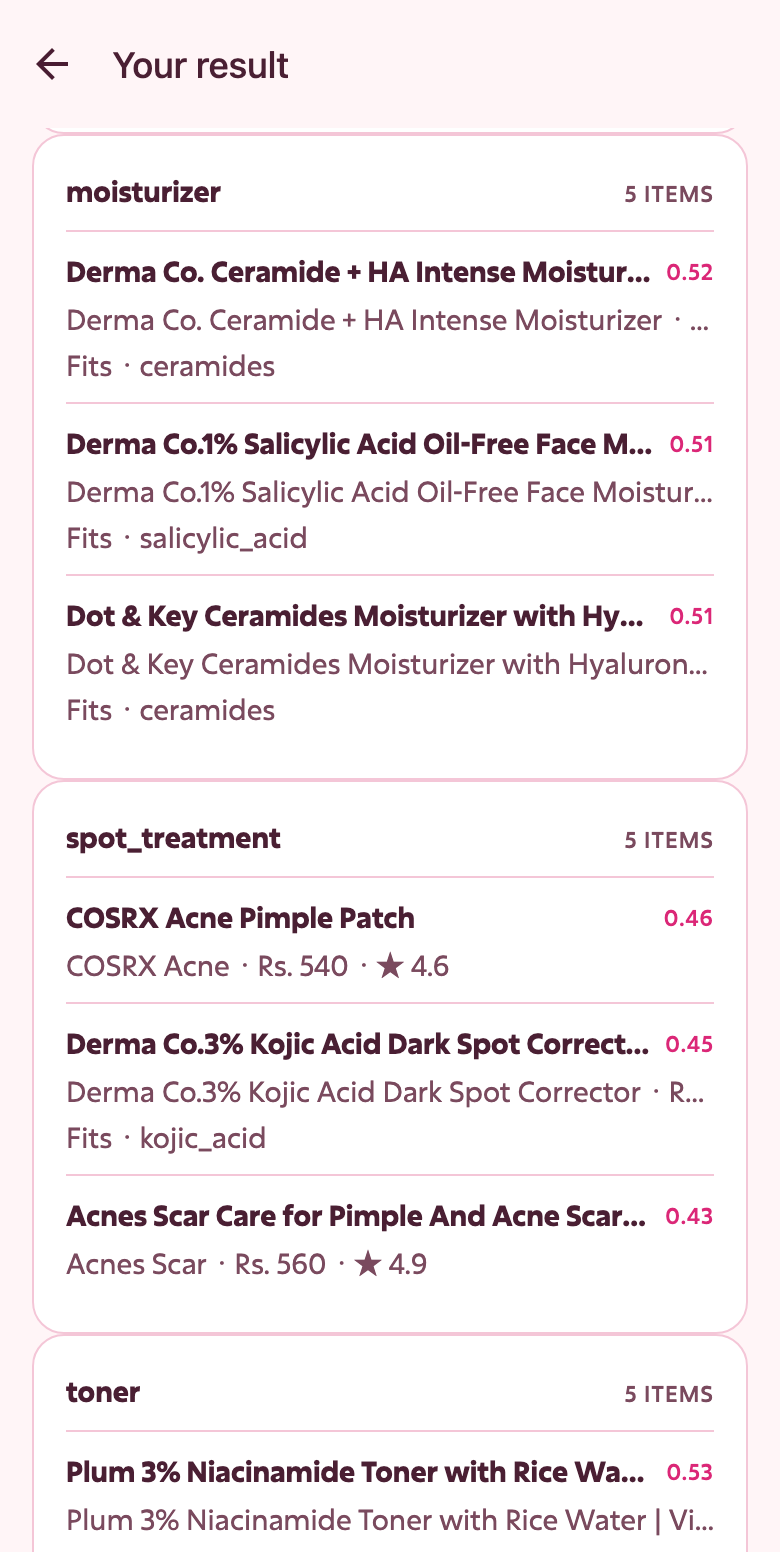
\includegraphics[width=\linewidth]{figures/analysis_2.png}\caption{More categories}\end{subfigure}
\caption{Screens from the running application (Expo web build, 390$\times$844 viewport). The analysed image is an FFHQ-Wrinkle test image.}
\label{fig:screens}
\end{figure}

\subsubsection*{Key development challenges}

Several practical problems consumed more time than planned. Each shaped the final design.

\begin{itemize}
  \item \textbf{Native photo upload.} On physical devices, photos selected in React Native could not be sent reliably as form data using the web-style \texttt{fetch} pattern. Uploads were rewritten to use \texttt{expo-file-system}. A 10\,MB size check was added on the client as well as the server, so that users receive an immediate, specific error rather than a generic failure.
  \item \textbf{Local networking.} The phone and the laptop running the backend must share a network, and the backend's address changes between networks. The client derives the server address from the Expo development host automatically. A ``Test connection'' diagnostic calls \texttt{/api/health} and reports exactly which URL failed. This turned a frequent source of confusion into a one-tap check.
  \item \textbf{Language-model integration.} Running Qwen2.5 inside the API process blocked other requests. Generation was moved to a worker thread behind an asynchronous lock. The analysis flow was made independent of the language model, and a rule-based fallback now answers when the model is slow, unavailable or returns invalid JSON.
  \item \textbf{Reproducibility.} After the preprocessing mismatch was discovered, a SHA-256 hash of the weights, the manifest paths and the preprocessing description were written into every evaluation file. This allows any reported number to be traced to the exact model and data that produced it.
\end{itemize}

These challenges map directly to the problem statement. Trustworthy guidance requires not only an accurate model, but also an application that fails clearly, explains its errors and can be reproduced.

\subsection{Validation and Testing}
\label{sec:validation}

Validation used five complementary kinds of evidence. All raw outputs are stored in \texttt{report/final/evidence/}.

\subsubsection*{Unit tests}

Nine test modules in \texttt{scripts/} were run. All passed, including a pipeline integration test that runs the real model and recommender end to end. Together they cover:
\begin{itemize}
  \item the API response contract;
  \item audit hashing;
  \item manifest and training logic (mask handling, balancing and non-overwrite);
  \item the SCIN quarantine;
  \item the language-model guardrail, which verifiably drops a fabricated product ID.
\end{itemize}
The suite is small, and only some of its checks are formal assertions.

\subsubsection*{Model performance on held-out data}

Table~\ref{tab:results} reports test metrics for the deployed \texttt{concern\_human\_reviewed} model. Thresholds were chosen on validation data. Figure~\ref{fig:results} compares F1, ROC-AUC and balanced accuracy, and Table~\ref{tab:modelcompare} compares all four model versions on the same test set.

\begin{table}[ht]
\centering\small
\caption{Held-out test performance of the deployed model (n = labelled test images per concern)}
\label{tab:results}
\setlength{\tabcolsep}{4pt}
\begin{tabular}{lrrrrrrrr}
\toprule
\textbf{Concern} & \textbf{n (+/--)} & \textbf{Thr.} & \textbf{Acc.} & \textbf{Prec.} & \textbf{Recall} & \textbf{F1} & \textbf{Bal.\,acc.} & \textbf{ROC-AUC}\\
\midrule
Blemishes & 101 (97/4) & 0.50 & 0.901 & 0.978 & 0.918 & 0.947 & 0.709 & 0.863\\
Dark spots & 87 (65/22) & 0.43 & 0.506 & 0.775 & 0.477 & 0.590 & 0.534 & 0.580\\
Redness & 105 (97/8) & 0.75 & 0.771 & 0.951 & 0.794 & 0.865 & 0.647 & 0.709\\
Visible pores & 55 (46/9) & 0.81 & 0.600 & 0.900 & 0.587 & 0.711 & 0.627 & 0.597\\
Fine lines & 234 (116/118) & 0.29 & 0.833 & 0.824 & 0.845 & 0.834 & 0.833 & 0.920\\
\midrule
\textbf{Macro} & 582 decisions & -- & 0.722 & 0.885 & 0.724 & \textbf{0.789} & \textbf{0.670} & \textbf{0.734}\\
\bottomrule
\end{tabular}

\vspace{2bp}{\footnotesize Pooled accuracy over all 582 known-label decisions: \textbf{76.3\%}. Macro PR-AUC: 0.904.}
\end{table}

\begin{figure}[ht]
\centering
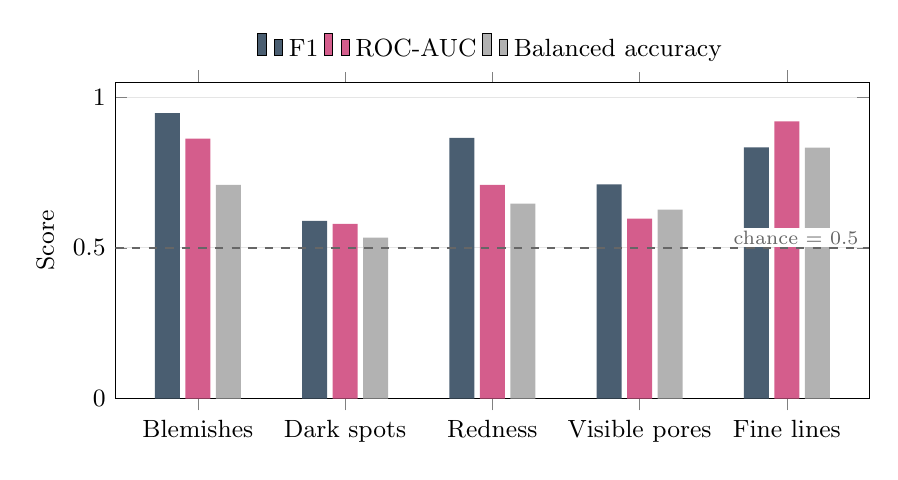
\begin{tikzpicture}
\begin{axis}[
  ybar, bar width=9bp, width=0.92\linewidth, height=5.6cm,
  ymin=0, ymax=1.05, ylabel={Score}, ylabel style={font=\small},
  symbolic x coords={Blemishes,Dark spots,Redness,Visible pores,Fine lines},
  xtick=data, x tick label style={font=\small},
  yticklabel style={font=\small}, ymajorgrids, grid style={black!10},
  legend style={at={(0.5,1.03)},anchor=south,legend columns=3,font=\small,draw=none},
  enlarge x limits=0.14]
\addplot[fill=TemplateBlue!75,draw=none] coordinates {(Blemishes,0.947)(Dark spots,0.590)(Redness,0.865)(Visible pores,0.711)(Fine lines,0.834)};
\addplot[fill=Accent!70,draw=none] coordinates {(Blemishes,0.863)(Dark spots,0.580)(Redness,0.709)(Visible pores,0.597)(Fine lines,0.920)};
\addplot[fill=black!30,draw=none] coordinates {(Blemishes,0.709)(Dark spots,0.534)(Redness,0.647)(Visible pores,0.627)(Fine lines,0.833)};
\draw[dashed,black!60] (rel axis cs:0,0.476) -- (rel axis cs:1,0.476) node[pos=0.99,font=\scriptsize,anchor=south east,fill=white,inner sep=1bp]{chance = 0.5};
\legend{F1, ROC-AUC, Balanced accuracy}
\end{axis}
\end{tikzpicture}
\caption{F1 overstates performance when positives dominate; ROC-AUC and balanced accuracy show where the model discriminates}
\label{fig:results}
\end{figure}

\begin{table}[ht]
\centering\small
\caption{All model versions on the same held-out test set (582 known-label decisions)}
\label{tab:modelcompare}
\begin{tabularx}{\linewidth}{P{3.6cm}rrrrY}
\toprule
\textbf{Model} & \textbf{Pooled acc.} & \textbf{Macro F1} & \textbf{Bal.\,acc.} & \textbf{ROC-AUC} & \textbf{Decision}\\
\midrule
\texttt{concern\_v2} (first labels) & 73.2\% & 0.779 & 0.635 & 0.717 & Replaced\\
Class-balanced candidate & 74.6\% & 0.736 & 0.617 & 0.708 & Rejected: redness specificity 0\\
\textbf{Human-reviewed (deployed)} & \textbf{76.3\%} & \textbf{0.789} & \textbf{0.670} & 0.734 & \textbf{Deployed}\\
Human-reviewed + MEMI melasma & 69.8\% & 0.701 & 0.662 & 0.750 & Rejected: accuracy fell\\
\bottomrule
\end{tabularx}
\end{table}

Three results stand out.
\begin{itemize}
  \item \textbf{Fine lines are learned well.} On the only balanced concern, the model reaches an ROC-AUC of 0.920 and a balanced accuracy of 0.833, up from 0.911 and 0.795.
  \item \textbf{More negative labels helped where they were added.} Redness accuracy rose from 55.2\% to 77.1\%, although its balanced accuracy barely changed (0.643 to 0.647). Blemish balanced accuracy rose from 0.610 to 0.709, and pores from 0.560 to 0.627. Even so, the test set still holds only 4 negative blemish images and 8 negative redness images, so these figures move by large steps when a single image changes. The high F1 scores for blemishes and redness still flatter the model: with 97 positives and 4 negatives, always saying ``present'' would give F1 $\approx$ 0.98.
  \item \textbf{Dark spots did not improve.} Dark-spot accuracy fell from 64.4\% to 50.6\% and ROC-AUC stayed at about 0.58. The deployed model is the best overall, but it is worse than \texttt{concern\_v2} on this one concern, and dark-spot output should be treated as unreliable.
\end{itemize}

\textbf{Run-to-run variation.} Training on the Apple GPU (tensorflow-metal) was not fully reproducible: retraining the same recipe with the same seed gave 72.2\% and 78.9\% macro accuracy. Over three runs, the human-reviewed recipe averaged 74.4\% macro accuracy and 0.746 ROC-AUC. Differences of a few points between single runs are therefore within noise. The deployed weights are the stored run whose metrics are reported above, identified by the SHA-256 hash in its evaluation file.

\textbf{Learning curve.} To test whether more data would help, the model was retrained on 25, 50, 75 and 100\% of the earlier gold training set (150 to 600+ images), with two seeds each (Figure~\ref{fig:lc}). ROC-AUC rose with data for blemishes (0.53 to 0.71) and pores (0.45 to 0.68). Dark spots stayed near 0.55. Fine lines were already at about 0.97 on that smaller, easier test set.

These trends suggest that more labelled data would help most concerns, but that dark spots may also need a better label definition. The run-to-run standard deviation (up to 0.20 for blemishes) is large relative to the gains, so these trends are indicative only.

\begin{figure}[ht]
\centering
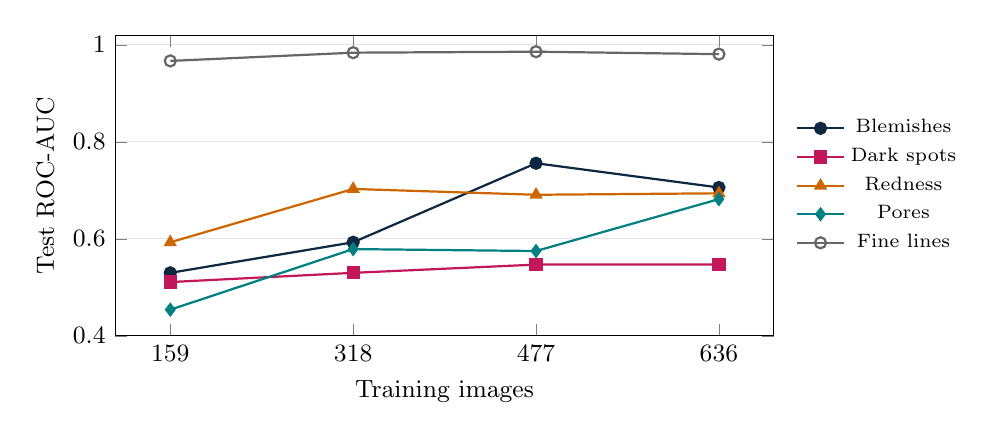
\begin{tikzpicture}
\begin{axis}[width=0.82\linewidth,height=5.4cm,xlabel={Training images},ylabel={Test ROC-AUC},
  xtick={159,318,477,636},ymin=0.4,ymax=1.02,ymajorgrids,grid style={black!10},
  legend style={font=\scriptsize,at={(1.02,0.5)},anchor=west,draw=none},
  label style={font=\small},tick label style={font=\small}]
\addplot[mark=*,TemplateBlue,thick] coordinates {(159,0.530)(318,0.593)(477,0.756)(636,0.706)};
\addplot[mark=square*,Accent,thick] coordinates {(159,0.511)(318,0.530)(477,0.547)(636,0.547)};
\addplot[mark=triangle*,orange!80!black,thick] coordinates {(159,0.593)(318,0.703)(477,0.691)(636,0.694)};
\addplot[mark=diamond*,teal,thick] coordinates {(159,0.454)(318,0.579)(477,0.575)(636,0.682)};
\addplot[mark=o,black!60,thick] coordinates {(159,0.967)(318,0.984)(477,0.986)(636,0.981)};
\legend{Blemishes,Dark spots,Redness,Pores,Fine lines}
\end{axis}
\end{tikzpicture}
\caption{Learning curve (mean of two seeds, earlier gold manifests)}
\label{fig:lc}
\end{figure}

\textbf{Negative experiments.} Two candidates were rejected (Table~\ref{tab:modelcompare}). Class reweighting slightly improved validation ROC-AUC (0.686 to 0.698), but on the test set macro F1 fell to 0.736 and redness specificity dropped to 0, with all eight negatives misclassified. Adding MEMI melasma photos raised macro ROC-AUC to 0.750 but lowered pooled accuracy to 69.8\% and left dark-spot ROC-AUC near chance (0.57). Both results point the same way: reweighting or adding positives cannot create the variety of \emph{negative} examples that is missing from the data.

\subsubsection*{Face-gate validation}

The YuNet gate (threshold 0.9) rejected all 300 PASCAL VOC non-face images. It was then run on every held-out test image to check how it would treat real inputs (Table~\ref{tab:gate}).

\begin{table}[ht]
\centering\small
\caption{Face-gate pass rate on held-out test images}
\label{tab:gate}
\begin{tabular}{lrrr}
\toprule
\textbf{Source / framing} & \textbf{Images} & \textbf{Passed} & \textbf{Rate}\\
\midrule
FFHQ-Wrinkle, full face & 211 & 211 & 100\%\\
Kaggle concerns, full face & 40 & 34 & 85\%\\
Original conditions, full face & 23 & 19 & 83\%\\
ACNE04, full face & 15 & 11 & 73\%\\
Kaggle concerns, close-up & 106 & 64 & 60\%\\
Original conditions, close-up & 54 & 14 & 26\%\\
ACNE04, close-up & 30 & 20 & 67\%\\
\midrule
\textbf{All} & 479 & 373 & \textbf{77.9\%}\\
\bottomrule
\end{tabular}
\end{table}

Of the held-out images, 22\% would be rejected by the deployed app before reaching the model. Most were facial close-ups, the framing that carries most of the blemish, pore and dark-spot labels. The model metrics therefore describe a wider input range than the app accepts. Conversely, the app never sees many of the close-ups on which the concern model was trained. This mismatch between the gate and the model is discussed in Section~\ref{sec:eval}.

\subsubsection*{Functional testing}

Nineteen black-box test cases were executed against the running API with \texttt{curl}. They were first run on 30 September 2026 and re-run on 1 October 2026 after the human-reviewed model was deployed. Appendix~\ref{app:tests} lists them in full, and Table~\ref{tab:funcsummary} summarises the re-run. Eighteen passed. One failed: TC15, the chat question. In the first run it returned a grounded reply after 55\,s. In the re-run it gave no response within 240\,s, and a retry also timed out after 500\,s. The cause is a design weakness: chat generations run one at a time behind a lock with no timeout, so a request that the client has abandoned keeps running and blocks every later one. Warm analysis latency over 10 runs had a median of 0.18\,s (maximum 0.24\,s) on an Apple M4 CPU, which satisfies N4.

\begin{table}[ht]
\centering\small
\caption{Functional test summary (details in Appendix~\ref{app:tests})}
\label{tab:funcsummary}
\begin{tabularx}{\linewidth}{lrrY}
\toprule
\textbf{Area} & \textbf{Cases} & \textbf{Pass} & \textbf{Observation}\\
\midrule
Analysis, valid input & 5 & 5 & Skin type correctly changes ranking (TC18/19); a false face rejection occurred in the first run (TC02)\\
Health \& input validation & 6 & 6 & Correct 400/422 codes; the corrupt-image message exposes an internal Python object name\\
Products \& metadata & 6 & 6 & Search, filter, 404 and categories correct\\
Chat & 2 & 1 & Empty message rejected; question answered in 55\,s in the first run but timed out in the re-run (TC15)\\
\midrule
\textbf{Total} & 19 & 18 & \\
\bottomrule
\end{tabularx}
\end{table}

\subsubsection*{Usability: heuristic evaluation}

The running application was first inspected against Nielsen's ten heuristics \citep{galavi2024}. The inspection used the screens in Figure~\ref{fig:screens} and a cognitive walkthrough of the ``check a photo, then read recommendations'' task. Severity was rated from 0 (not a problem) to 4 (catastrophe). Because the evaluator also built the system, problems may be missed or rated leniently, so these findings are complemented by the participant survey below.

\begin{table}[ht]
\centering\small
\caption{Heuristic evaluation findings (author-conducted; severity 0--4)}
\label{tab:heuristic}
\begin{tabularx}{\linewidth}{P{3.3cm}Yc}
\toprule
\textbf{Heuristic} & \textbf{Finding} & \textbf{Sev.}\\
\midrule
Match with real world & The evening routine lists ``broad-spectrum sunscreen'' because the routine is split into morning and evening by position, not by step type & 3\\
Aesthetic \& minimalist & Chat replies show raw Markdown (\texttt{**bold**}) instead of formatted text & 2\\
Consistency \& standards & Settings chips truncate labels (``Not provided'' is clipped; ``Combination'' and ``Sensitive'' overlap) on a 390\,px screen & 2\\
Consistency \& standards & The About panel lists ``Jeevee $\cdot$ Oriflame'' but omits ForEveryNG, which supplies 41\% of products & 1\\
Error prevention & Close-up photos are rejected with ``No face found'' although the concern model can analyse them & 3\\
Visibility of system status & Chat gives no progress indication during a response that can take about 55\,s on CPU & 2\\
Help users with errors & Rejections give an actionable retake instruction; network errors are translated into plain language & 0\\
Recognition vs.\ recall & Score bars show a threshold tick and a status label, so users need not remember what a score means & 0\\
Accuracy of content & Some products sit in the wrong category (a body wash appears under ``toner'') because of keyword categorisation & 2\\
Code quality (dev) & React warning: \texttt{<button>} nested in \texttt{<button>} on the history and result screens (invalid markup; accessibility risk) & 1\\
\bottomrule
\end{tabularx}
\end{table}

\subsubsection*{Usability: participant survey}
\label{sec:survey}

Participants used the app on their own phones and then completed an anonymous Google Form (protocol and questions in Appendix~\ref{app:usability}). Each participant carried out four tasks: check a face photo, read and interpret the result, find and save a recommended product, and ask the assistant a question. For each task they reported whether they completed it and rated its ease from 1 (very difficult) to 5 (very easy). They then completed the ten-item System Usability Scale (SUS), scored from 0 to 100, where about 68 is the usual benchmark for average usability \citep{vlachogianni2022}. Finally, they answered questions on whether they understood the ``uncertain'' label, noticed the disclaimer, and would trust or buy the recommended products. Responses were exported from Google Forms as CSV and analysed with a script stored in \texttt{evidence/user\_study/}.

% TODO(user): fill from the exported responses CSV -- run
%   python3 evidence/user_study/analyse_sus.py responses.csv
% and paste the real figures below. Do not invent values.
\begin{table}[ht]
\centering\small
\caption{Participant survey results (n = [TODO])}
\label{tab:survey}
\begin{tabularx}{\linewidth}{lY}
\toprule
\textbf{Measure} & \textbf{Result}\\
\midrule
Participants & [TODO: n, age bands, skin types]\\
Task 1: check a photo & [TODO: completion \%, mean ease]\\
Task 2: read the result & [TODO]\\
Task 3: find and save a product & [TODO]\\
Task 4: ask the assistant & [TODO]\\
SUS score & [TODO: mean (SD), range]\\
Understood ``uncertain'' & [TODO: \% yes]\\
Noticed disclaimer & [TODO: \% yes]\\
Would trust / buy recommendations & [TODO: mean 1--5]\\
\bottomrule
\end{tabularx}
\end{table}

[TODO: two or three sentences summarising the main themes from the open comments, quoting participants only with their permission.]


\section{Critical Evaluation}
\label{sec:eval}

SkinCare AI is a working, end-to-end prototype. A user photographs their face and receives a per-concern cosmetic observation with its uncertainty. They can add their skin type and get a short list of products that are in stock at Nepalese retailers, with the reason each was chosen. They can then ask follow-up questions of an assistant that is not allowed to invent products.

This section judges how well the artefact meets its objectives and requirements, how far its evaluation can be trusted, how it compares with the systems reviewed in Section~\ref{sec:lit}, and what the project process itself taught.

\subsection*{Achievement of objectives}

\begin{table}[ht]
\centering\small
\caption{Objective attainment}
\label{tab:objectives}
\begin{tabularx}{\linewidth}{lcY}
\toprule
\textbf{Objective} & \textbf{Status} & \textbf{Evidence and judgement}\\
\midrule
O1 Dataset & Met & 26,000+ images audited; 1,400+ reviewed, plus a second review of 200 training images; 2,000+ images in leakage-free splits. Test negatives remain scarce for three concerns.\\
O2 Model & Partly met & Four versions trained and compared on one fixed test set; the best (pooled accuracy 76.3\%, macro F1 0.789) is deployed. Fine lines are strong (ROC-AUC 0.920); blemishes and redness moderate; dark spots and pores near chance.\\
O3 Catalogue & Met & 1,500+ products from 3 retailers, above the target of 1,000. Ingredient tags cover only 35\% of products.\\
O4 Recommender & Met & Transparent weighted ranking that responds to skin type (TC18/19) and shows matched ingredients. Its suitability has not been rated by experts.\\
O5 Application & Met & All F1--F10 requirements implemented, four only partly met (Table~\ref{tab:reqcheck}); 18 of 19 functional tests passed.\\
O6 Evaluation & Met & Model metrics, learning curve, 19 functional tests, heuristic review and a participant SUS survey. No fresh, never-inspected test set.\\
\bottomrule
\end{tabularx}
\end{table}

\subsection*{Requirements check}

Table~\ref{tab:reqcheck} checks every requirement in Table~\ref{tab:spec} against the test evidence. All requirements are present; four are only partly met because testing exposed a specific weakness.

\begin{table}[ht]
\centering\small
\caption{Requirements against evidence}
\label{tab:reqcheck}
\begin{tabularx}{\linewidth}{lcY}
\toprule
\textbf{Req.} & \textbf{Status} & \textbf{Evidence}\\
\midrule
F1 Upload & Met & TC05, TC07: wrong type and oversize files rejected with clear messages\\
F2 Face gate & Partly & All 300 non-face images rejected (TC04), but 22\% of held-out close-ups also rejected (Table~\ref{tab:gate})\\
F3 Per-concern status & Met & TC02, TC03: score, threshold and status for all five concerns\\
F4 Skin type & Met & TC17--TC19: invalid type rejected; valid type changes the ranking\\
F5 Recommendations & Met & Up to five products per category with matched ingredients\\
F6 Routine & Partly & Routine shown, but sunscreen can appear in the evening (Table~\ref{tab:heuristic})\\
F7 Catalogue & Met & TC09--TC13: search, filter, sort, detail and 404\\
F8 History & Met & On-device history under the Saved tab (Figure~\ref{fig:screens})\\
F9 Chat & Partly & Grounded replies in the first run, but no timeout: queued requests blocked the re-run (TC15)\\
F10 Disclaimer & Met & Shown on result and chat screens\\
\midrule
N1 No medical labels & Met & Only cosmetic concerns; red-flag questions are signposted to a dermatologist\\
N2 Validation-only thresholds & Met & Thresholds stored with their validation source in \texttt{evaluation.json}\\
N3 No photo storage & Met & Server is stateless; history kept on the device\\
N4 Analysis under 2\,s & Met & Warm analysis well under 1\,s (Section~\ref{sec:validation})\\
N5 Free software only & Met & No paid APIs; Qwen2.5 runs locally\\
N6 Structured errors & Partly & Correct codes, but the corrupt-image message exposes an internal object name (TC06)\\
\bottomrule
\end{tabularx}
\end{table}

\subsection*{Model results}

The central technical result is mixed, and it should be stated plainly. The deployed model is \emph{useful for fine lines}, \emph{moderate for blemishes and redness}, and \emph{not yet useful for dark spots or visible pores}. The interim target of a weighted F1 of at least 80\% was, in effect, replaced. A macro F1 of 0.789 could be presented as ``close to target''. That would be misleading, because F1 rewards always predicting ``present'' when positives far outnumber negatives \citep{chicco2020}. Reporting accuracy, balanced accuracy and ROC-AUC next to F1 is less flattering but truthful.

The sequence of model versions (Table~\ref{tab:modelcompare}) is the clearest evidence in the project about what limits performance:
\begin{itemize}
  \item \textbf{Changing the loss did not help.} Class reweighting targets imbalance directly, yet it lowered test F1 and reduced redness specificity to zero.
  \item \textbf{Adding more positives did not help.} Extra melasma photos raised ROC-AUC slightly but lowered accuracy, and dark spots stayed near chance.
  \item \textbf{Adding reviewed negatives did help.} Filling unknown labels in existing training images raised the number of negative training labels from 9 to 159 for blemishes and from 19 to 188 for redness. This produced the only candidate that improved all four macro metrics, with the largest gains on exactly those concerns.
\end{itemize}
Together with the learning curve (Figure~\ref{fig:lc}), which was still rising for most concerns, these results show that the bottleneck is the quantity and variety of labelled data, especially negatives, and not the network.

The improvement must also be kept in proportion. It is a single stored training run, and same-seed retraining varied by several points on the Apple GPU. The averaged runs still favour the human-reviewed recipe, but the margin over \texttt{concern\_v2} is modest. The deployed model is also worse than \texttt{concern\_v2} on dark spots, so the replacement was a trade-off, made because it was better overall and on the concerns with the largest gains.

\subsection*{Validity of the evaluation}

Four threats to validity must be acknowledged.

\begin{itemize}
  \item \textbf{The test set is no longer untouched.} Its results were inspected while comparing four model versions. No threshold was ever set on test data, but choosing the deployed model by comparing test results is a form of selection. The set should now be treated as a regression benchmark, and a fresh independent test set is needed for final claims about generalisation.
  \item \textbf{Very small negative counts.} The test set has only 4 negative blemish images and 8 negative redness images. One image more or less changes specificity by 12 to 25 points, so per-concern balanced accuracy for these concerns is unstable.
  \item \textbf{The test population differs from the app's inputs.} The face gate rejects 22\% of test images (Table~\ref{tab:gate}), mostly close-ups. The metrics therefore describe a broader input range than the app accepts.
  \item \textbf{Representation is unmeasured.} No image carries a skin-tone label, so it is unknown how the model performs on Nepalese users. Given \citet{groh2021}, \citet{daneshjou2021} and \citet{daneshjou2022}, a performance gap for darker skin should be assumed until measured.
\end{itemize}

\subsection*{Recommender quality}

The recommender behaves as designed, but its inputs are thin. Only 35\% of products have an inferred target ingredient, so for most candidates the 0.40 ingredient weight contributes nothing. The ranking then falls back on rating and review count, which rewards popular products rather than suitable ones. Keyword categorisation also misplaces some products; for example, a body wash appears in the toner list.

On the positive side, every recommendation can be explained line by line, and stock status and price come from real retailers. Changing the stated skin type visibly changes the ranking: ceramide moisturisers rise for dry skin and oil-free ones for oily skin (TC18/19). No dermatologist has yet judged whether the recommendations are \emph{appropriate}, so clinical suitability remains unvalidated.

\subsection*{Usability}

The heuristic review found two severity-3 problems: sunscreen listed in the evening routine, and close-up photos rejected with ``No face found''. Both were confirmed by other evidence (the routine logic and the face-gate test), so they are real defects rather than evaluator opinion. The remaining issues were cosmetic or minor.

The participant survey (Section~\ref{sec:survey}, Table~\ref{tab:survey}) adds the user's view. [TODO: after the responses are analysed, state the mean SUS score against the benchmark of 68 \citep{vlachogianni2022}, the task with the lowest completion or ease rating, and whether participants understood the ``uncertain'' label and the disclaimer. Note whether the survey confirmed the heuristic findings.]

\subsection*{Comparison with existing systems}

The artefact differs from the systems reviewed in Section~\ref{sec:lit} in four ways.

\begin{enumerate}
  \item \textbf{Scope honesty.} Clinical systems such as \citet{liu2020}, and most of those reviewed by \citet{jones2022}, target diagnosis using curated clinical data. This project deliberately removed diagnosis after finding that its data could not support it. It presents outputs as observations with an \emph{uncertain} band, so the system fails visibly rather than confidently.
  \item \textbf{Leakage-aware data engineering.} Many applied skin projects built on Kaggle data report accuracy without controlling for duplicates. This project grouped duplicates across splits, recorded provenance for every source, kept every model version, and published negative results. Its numbers are lower, but they mean what they claim \citep{kapoor2023}.
  \item \textbf{Local market grounding.} Unlike the global recommenders reviewed by \citet{ramrakhiani2024}, every product suggested is sold by a Nepalese retailer, priced in rupees and marked with its stock status.
  \item \textbf{Code-enforced language-model grounding.} The assistant can only mention catalogue products. This is enforced in code rather than by the prompt alone, which directly limits the hallucination risk described by \citet{ji2023}.
\end{enumerate}

Compared with the interim design, Grad-CAM heatmaps and TF-IDF similarity were not implemented. The explainability gap identified in the interim report is therefore only partly closed: the system offers transparent scores and reasons, but no visual attribution.

\subsection*{Reflection on the project process}

The most valuable decision was to stop tuning the first model and audit the data instead. It cost several weeks and forced a change of scope, but without it the project would have reported high accuracy on leaked, mislabelled data. The iterative process made this change possible. Its cost was time: the second label review, the experiments and the user survey all happened late, leaving no time to collect a new, independent test set. With hindsight, the data audit should have been the first task of the project rather than a response to poor results, and label review should have targeted negative examples from the start.

\subsection{Impact}

\textbf{For Nepalese consumers,} the prototype shows that a free, phone-based first step is feasible. It gives cosmetic guidance tied to purchasable products and a clear signpost to a dermatologist. Its current accuracy does \emph{not} justify public release. Its greatest potential impact is as a validated pipeline into which better data can be fed.

\textbf{For Nepalese e-commerce,} the unified catalogue and recommender could help retailers such as Jeevee or ForEveryNG guide customers to in-stock products by need rather than by brand. The catalogue audit also shows that most listings omit ingredient information. Retailers could fix this cheaply, and doing so would improve both search and recommendation.

\textbf{For academic practice,} the project provides a documented, reproducible example of how aggregated public skin data can mislead. More than half of the images were near-duplicates, and 2,400+ duplicate groups spanned sources. It also shows that targeted human review of negatives improved the model more than changing the loss or adding positives. This supports calls for transparent documentation of datasets and their limitations \citep{gebru2021}.

\textbf{Ethically,} the pivot away from disease labels reduces the risk of false reassurance. With the earlier design, a user with a serious lesion might have trusted a ``no carcinoma'' result. The residual risk is that users over-trust cosmetic outputs. This is mitigated, but not eliminated, by uncertainty display and disclaimers.

\section{Conclusion}
\label{sec:conclusion}

This project set out to give Nepalese users trustworthy skincare guidance from a single photograph, linked to products they can actually buy. It delivered a complete mobile prototype. A YuNet face gate, a multi-label EfficientNetB0 concern model, a catalogue of 1,500+ Nepalese products, a transparent weighted recommender and a grounded Qwen2.5 assistant are integrated behind a FastAPI backend and an Expo client.

The most important moment in the project was not a modelling choice but a data audit. The audit revealed that the original data was dominated by duplicates, stock imagery and unverifiable labels. On that evidence the scope was narrowed: from diseases and photo-based skin type to five human-labelled cosmetic concerns. This made the system safer and its results meaningful.

Those results are modest but improving. Four model versions were compared on one fixed held-out set. The deployed model, retrained after a second review that added many negative labels, reached a pooled accuracy of 76.3\%, a macro F1 of 0.789 and a macro ROC-AUC of 0.734, the best of the four. Fine lines are detected reliably (ROC-AUC 0.920), blemishes and redness moderately, and dark spots and visible pores barely better than chance. Reweighting the loss and adding melasma photos both failed, while adding reviewed negatives helped, which confirms that the limiting factor is the data. Eighteen of 19 functional tests passed; the chat assistant timed out when requests queued. Testing also exposed a mismatch between the face gate and the model, and several interface defects that are now documented.

The project therefore succeeds as an engineering artefact and as an honest baseline. It does not yet succeed as a consumer product. Its value lies in a working pipeline from photo to purchasable product, a reproducible leakage-aware protocol, and a clear, evidence-based account of what must improve next.

\subsection{Limitations}

\begin{description}[leftmargin=0pt,style=nextline]
  \item[Too few test negatives and no skin-tone labels.] The test set has only 4, 8 and 9 negative images for blemishes, redness and pores. A single image changes their specificity by 11 to 25 points. Nothing is known about performance by skin tone. \emph{Impact:} claims beyond fine lines are weak, and fairness is unmeasured. \emph{Addressed by:} reporting balanced accuracy and ROC-AUC next to F1, and stating the gap explicitly.
  \item[Test set reused for model choice.] The same test set was inspected while comparing four model versions, and the deployed model was chosen partly on those results. \emph{Impact:} the reported metrics are a regression benchmark, slightly optimistic, and not an independent estimate. \emph{Addressed by:} never setting thresholds on test data, and flagging the issue.
  \item[Training not fully reproducible.] On the Apple GPU, the same recipe and seed gave 72.2\% and 78.9\% macro accuracy. \emph{Impact:} differences of a few points between single runs are within noise, so the gain over \texttt{concern\_v2} is modest. \emph{Addressed by:} storing each deployed model's weight hash and reporting averaged runs.
  \item[Dark-spot regression.] The deployed model is worse than \texttt{concern\_v2} on dark spots (accuracy 50.6\% versus 64.4\%), and no version separates dark spots well. \emph{Impact:} dark-spot output is unreliable and should not drive recommendations on its own.
  \item[Labels from one reviewer, and not new data.] All human labels come from a single reviewer, and inter-rater agreement was not measured. The second review re-labelled existing training images rather than adding new people. \emph{Impact:} label noise is unknown, and the data's variety did not grow.
  \item[Gate--model mismatch.] 22\% of test images, mostly close-ups, would be rejected by the app. \emph{Impact:} users who photograph close-ups are turned away, and the metrics cover inputs the app does not accept.
  \item[Sparse catalogue metadata.] 65\% of products have no inferable target ingredient, and 18\% have no category. \emph{Impact:} the ranking leans on popularity, and some products appear in the wrong category.
  \item[Small, self-selected survey.] Survey participants were a convenience sample recruited by the author, used the app briefly and unsupervised, and rated perceived usability only. \emph{Impact:} the results show first impressions, not long-term use, and cannot judge whether the observations or recommendations are correct.
  \item[Chat latency and prototype hosting.] CPU-based language-model responses take about a minute, requests are processed one at a time with no timeout, and the system runs only on a local network.
\end{description}

\subsection{Future Work}

\begin{enumerate}
  \item \textbf{Collect targeted negatives and a fresh test set.} This is the highest priority. With ethics approval and consent, collect full-face photos from Nepalese volunteers across Fitzpatrick types, deliberately including people \emph{without} each concern. Hold out a new test set that is never inspected during development, and report metrics by skin tone \citep{groh2021}.
  \item \textbf{Measure label reliability.} Have a second annotator, ideally with cosmetology or dermatology training, label a subset, and report Cohen's $\kappa$ for each concern. Revise the definition for dark spots, where every model version stayed near chance.
  \item \textbf{Make training reproducible.} Train final models with deterministic settings (or on CPU) and report the mean and spread over several seeds rather than a single run.
  \item \textbf{Align the gate and the model.} Either train and evaluate only on full-face images, or accept close-ups with a separate quality check. Report metrics on exactly the images the app accepts.
  \item \textbf{Fix the defects found in testing.} Assign routine steps to morning or evening by step type, render Markdown in chat, fix the chip layout and nested buttons, sanitise the corrupt-image message, and add a progress indicator and a timeout to chat, so an abandoned request cannot block later ones.
  \item \textbf{Enrich the catalogue.} Scrape full INCI ingredient lists where available, validate categories with a small classifier, and test whether embedding similarity then beats the weighted rules using expert-rated relevance (for example, precision@5).
  \item \textbf{Extend the user study.} Repeat the survey with a larger and more varied sample, including older users and people outside Kathmandu, add observed (moderated) sessions, and iterate on the findings.
  \item \textbf{Add visual explanation and deployment.} Add Grad-CAM overlays \citep{selvaraju2020} for concerns marked \emph{present}. Export the model to TensorFlow Lite for on-device inference, which also improves privacy, and add Nepali-language support.
\end{enumerate}


% ================= REFERENCES =================
\clearpage
\renewcommand{\bibname}{References}
\renewcommand{\refname}{References}
\bibliographystyle{agsm}
\phantomsection
\addcontentsline{toc}{section}{References}
\bibliography{references}

% ================= APPENDICES =================
\clearpage
\appendix
\renewcommand{\thesection}{\Alph{section}}
\titleformat{\section}{\fontsize{16bp}{20bp}\selectfont\bfseries}{Appendix \thesection:}{0.5em}{}
\renewcommand{\cftsecaftersnum}{}
\addtocontents{toc}{\protect\renewcommand{\protect\cftsecaftersnum}{}\protect\setlength{\protect\cftsecnumwidth}{1.6em}}
\setlength{\cftsecnumwidth}{1.6em}
\addcontentsline{toc}{section}{Appendices}

\section{Project Timeline}
\label{app:timeline}

Figure~\ref{fig:gantt} shows the actual schedule. Dates from August 2026 onwards are taken from the Git history. Earlier dates follow the interim report's plan.
% TODO(Krishu): confirm the January-July dates against your own records.

\begin{figure}[ht]
\centering
\resizebox{\linewidth}{!}{%
\begin{ganttchart}[
  hgrid, vgrid, x unit=0.95cm, y unit chart=0.52cm,
  title height=1, bar height=0.55,
  bar/.append style={fill=TemplateBlue!65,draw=none},
  group/.append style={fill=Accent!80,draw=none},
  milestone/.append style={fill=Accent,draw=none},
  bar label font=\small, group label font=\small\bfseries, milestone label font=\small\itshape,
  title label font=\small\bfseries]{1}{10}
\gantttitle{2026}{10}\\
\gantttitle{Jan}{1}\gantttitle{Feb}{1}\gantttitle{Mar}{1}\gantttitle{Apr}{1}\gantttitle{May}{1}\gantttitle{Jun}{1}\gantttitle{Jul}{1}\gantttitle{Aug}{1}\gantttitle{Sep}{1}\gantttitle{Oct}{1}\\
\ganttgroup{Research \& planning}{1}{5}\\
\ganttbar{Literature review, proposal}{1}{3}\\
\ganttbar{Interim design and report}{3}{5}\\
\ganttmilestone{Interim report (5 May)}{5}\\
\ganttgroup{Data \& catalogue}{3}{9}\\
\ganttbar{Product scraping and enrichment}{3}{6}\\
\ganttbar{Kaggle image collection}{4}{7}\\
\ganttbar{Vision data audit and review}{9}{9}\\
\ganttgroup{Development}{6}{9}\\
\ganttbar{Multi-task prototype, SLM}{7}{8}\\
\ganttbar{Mobile app and API}{8}{9}\\
\ganttmilestone{Progress review (8 Sep)}{9}\\
\ganttbar{Concern model v1, v2 (FFHQ)}{9}{9}\\
\ganttgroup{Evaluation \& writing}{9}{10}\\
\ganttbar{Testing, experiments}{9}{10}\\
\ganttbar{Final report}{9}{10}\\
\ganttmilestone{Final submission (date TBD)}{9}
\end{ganttchart}}
\caption{Project Gantt chart}
\label{fig:gantt}
\end{figure}

\section{Feasibility, Risks, and Ethical Aspects}

\subsection*{B.1 Revised Feasibility}

The project proved feasible within its revised scope.
\begin{itemize}
  \item All software is free and open source.
  \item Training fits on a laptop, because EfficientNetB0 with 1,200+ images trains in minutes per phase on an Apple M-series CPU.
  \item Analysis runs in under 0.25\,s once the model is loaded.
\end{itemize}

The binding constraints were the following:
\begin{itemize}
  \item \emph{Labelled data}: human review is slow, and public cosmetic datasets are small.
  \item \emph{Time}: the September pivot left little time for the participant study and no time to collect a new test set.
  \item \emph{Compute for the language model}: CPU chat responses take about a minute.
\end{itemize}
The core flow does not depend on the language model, so this last constraint did not threaten delivery.

\subsection*{B.2 Updated Risk Analysis and Mitigation}

\begin{table}[ht]
\centering\small
\caption{Risk assessment and mitigation (updated with outcomes)}
\label{tab:risks}
\begin{tabularx}{\linewidth}{P{3.2cm}ccY}
\toprule
\textbf{Potential risk} & \textbf{Likelihood} & \textbf{Impact} & \textbf{Mitigation strategy and outcome}\\
\midrule
Small or contaminated dataset causing misleading accuracy & High & High & Audited duplicates, split by duplicate group, human review. \emph{Occurred}; mitigated by the scope change and honest metrics.\\
Poor performance on Nepalese skin tones & High & High & Report as unmeasured; plan skin-tone-stratified collection. \emph{Open.}\\
Language model hallucinating products or ingredients & Medium & High & Candidate-only prompt, code-level ID validation, rule fallback. \emph{Mitigated} (guardrail test passes).\\
Users treating output as diagnosis & Medium & High & No disease labels, ``uncertain'' band, persistent disclaimer. \emph{Reduced.}\\
Scraper blocked or site layout changes & Medium & Medium & Snapshot CSVs kept; three independent sources. \emph{Did not occur.}\\
Language-model latency too high & High & Low & Made optional; rule fallback. \emph{Occurred} (about 55\,s); core flow unaffected.\\
Insufficient time for user study & High & Medium & Short online survey (Google Forms) alongside a heuristic review. \emph{Mitigated}; sample is small.\\
\bottomrule
\end{tabularx}
\end{table}

\subsection*{B.3 Revised Ethical Considerations}

\textbf{Human participants.} The usability survey followed the protocol in Appendix~\ref{app:usability}. Participants were adults who gave informed consent on the first page of the form. The form collected no names, emails or photos, and participants could use a sample photo instead of their own. Any photo used in the app is processed in memory and never stored. [TODO: state the ethics approval or supervisor sign-off obtained before the survey was sent.]

\textbf{Third-party data.} Every image source was recorded with its licence. Sources with unclear provenance were rejected or limited to partial use. FFHQ-Wrinkle (CC BY-NC-SA) and ACNE04 (academic use) are used non-commercially with attribution. SCIN images were downloaded under the SCIN Data Use Licence, which prohibits re-identification. Their privacy masks were left untouched, and the images were quarantined unused. Raw images are not committed to the repository.

\textbf{Scraping.} Only publicly listed product information was collected, at a low request rate, for non-commercial academic use. No customer data was collected.

\textbf{Privacy in the app.} Uploaded photos are processed in memory and are not stored on the server. Scan history and favourites stay on the user's device.

\textbf{Harm and fairness.} Removing disease labels avoids false medical reassurance. Every result states that it is a cosmetic observation and not a diagnosis. The known risk of lower accuracy on under-represented skin tones is stated openly rather than hidden \citep{daneshjou2021,groh2021}. A public release should wait until performance has been measured on the intended population.

\textbf{Academic integrity.} All reported numbers come from stored evaluation files or recorded test outputs. Heuristic findings are labelled as author-conducted, and survey results are taken only from the exported Google Forms responses, analysed with the script in \texttt{evidence/user\_study/}.

\section{Functional Test Cases}
\label{app:tests}

These cases were first executed on 30 September 2026 and re-run on 1 October 2026 after the human-reviewed model was deployed. The table shows the re-run (raw output in \texttt{evidence/}; the first run is kept alongside it with the suffix \texttt{\_20260930}).

{\small
\begin{longtable}{P{0.9cm}P{3.8cm}P{3.3cm}P{3.4cm}P{1.2cm}}
\toprule
\textbf{ID} & \textbf{Input} & \textbf{Expected} & \textbf{Actual} & \textbf{Result}\\
\midrule\endhead
TC01 & GET /api/health & 200, status ok & 200, status ok & Pass\\
TC02 & ACNE04 face image, skin type oily & 200, concerns and recommendations & 200; 3 present, 2 absent; 6 categories $\times$ 5 & Pass$^\dagger$\\
TC03 & FFHQ face, no skin type & 200, 5 concerns, recommendations & 200; fine lines present, 4 absent; 4 categories $\times$ 5 & Pass\\
TC04 & PASCAL VOC boat photo & 200, rejected, retake message & 200, rejected, retake message & Pass\\
TC05 & Text file (text/plain) & 400 ``File must be an image'' & 400 as expected & Pass\\
TC06 & Corrupt bytes labelled image/jpeg & 422 & 422, message exposes Python object name & Pass*\\
TC07 & 11\,MB file & 400 ``Image too large'' & 400 as expected & Pass\\
TC08 & Missing image field & 422 & 422 field required & Pass\\
TC09 & List products, page size 5 & 200, 5 products & 200, 5 products & Pass\\
TC10 & Filter sunscreen + oily & 200, matching products & 200, SPF gel products & Pass\\
TC11 & Search ``niacinamide'' & 200, relevant products & 200, niacinamide products & Pass\\
TC12 & Unknown product ID & 404 & 404 ``Product not found'' & Pass\\
TC13 & GET categories & 200, category list & 200, 11 categories & Pass\\
TC14 & GET skin types & 200, 5 skin types & 200, with ingredients & Pass\\
TC15 & Chat ``What helps with dark spots?'' & 200, grounded reply & No response within 240\,s (first run: grounded reply in 54.9\,s) & \textbf{Fail}\\
TC16 & Chat with empty message & 422 & 422 string too short & Pass\\
TC17 & Invalid skin type ``purple'' & 422 & 422 ``Unknown skin type'' & Pass\\
TC18 & FFHQ face, skin type dry & Ranking favours dry-skin products & Ceramide moisturisers ranked top & Pass\\
TC19 & Same face, skin type oily & Ranking favours oily-skin products & Oil-free moisturisers ranked top & Pass\\
\bottomrule
\end{longtable}
}
{\footnotesize *Passed with an observation recorded in Table~\ref{tab:funcsummary}. $^\dagger$In the first run a different ACNE04 image was wrongly rejected by the face gate; the gate is unchanged, so such false rejections still occur (Table~\ref{tab:gate}).}

\section{Annotation Guide and Usability Study Protocol}
\label{app:annotation}
\label{app:usability}

\subsection*{D.1 Annotation guide (summary)}

Reviewers mark only what is visibly supported by the image. \emph{Unknown} is used whenever framing, lighting, resolution, makeup or occlusion prevents a judgement. Uncertainty is never converted to \emph{absent}. An image is marked unusable if any of the following applies:
\begin{itemize}
  \item it is not facial skin;
  \item it is a collage or heavily edited;
  \item it has a dominant watermark;
  \item it is badly exposed.
\end{itemize}

\begin{tabularx}{\linewidth}{lYY}
\toprule
\textbf{Label} & \textbf{Present when} & \textbf{Not sufficient alone}\\
\midrule
Blemishes & Visible pimples, inflamed spots, blackheads or whiteheads & Scars or pigmentation without active blemishes\\
Dark spots & Localised darker marks or visibly uneven pigmentation & Shadows, freckles alone, lighting gradients\\
Redness & Redness distinguishable from normal tone & Warm lighting, blush, colour cast\\
Visible pores & Clearly visible pores at usable resolution & Compression noise, extreme zoom texture\\
Fine lines & Clearly visible fine lines or wrinkles & Folds caused by a single exaggerated expression\\
\bottomrule
\end{tabularx}

\subsection*{D.2 Usability survey protocol}

\textbf{Participants:} adults living in Nepal, recruited by convenience sampling from the author's contacts, with varied skin types. Participation was voluntary and anonymous.

\textbf{Procedure} (about 20 minutes per participant):
\begin{enumerate}
  \item Participant opens the Google Form and gives consent on its first page.
  \item Participant opens SkinCare AI (Expo build on the same network as the backend) and optionally sets a skin type.
  \item Task 1: check one face photo. A sample photo is offered, so using their own image is optional.
  \item Task 2: open the result and read what each concern means.
  \item Task 3: find a recommended product and save it to the shelf.
  \item Task 4: ask the assistant one question about the result.
  \item Participant completes the rest of the form: task completion and ease, the ten SUS items, understanding and trust questions, and open comments.
\end{enumerate}

\textbf{Form sections} (created by \texttt{evidence/user\_study/create\_form.gs}):
\begin{enumerate}[label=\arabic*.,itemsep=0pt]
  \item Information and consent (required).
  \item About you: age group, self-reported skin type, prior use of skincare apps, own or sample photo.
  \item Tasks 1--4: completed (yes without help / yes with help / no) and ease (1--5).
  \item System Usability Scale, ten items \citep{vlachogianni2022}.
  \item Understanding and trust: meaning of ``uncertain'' (multiple choice), disclaimer noticed, results match what is visible, trust in recommendations, usefulness of ingredient reasons, intention to buy (1--5 each).
  \item Open comments: what was liked, what was confusing.
\end{enumerate}

\textbf{Analysis:} the responses CSV is processed by \texttt{analyse\_sus.py}, which computes each participant's SUS score (odd items $r-1$, even items $5-r$, sum $\times 2.5$), the mean and standard deviation, task completion rates, mean ease ratings and answer counts.

\textbf{Consent statement:} ``Taking part is voluntary and you may stop at any time without giving a reason. Any photo you use in the app is analysed in memory and is not stored. Your answers are anonymous and will be used only in the project report. The app gives cosmetic observations, not medical advice.''

\textbf{SUS items} (rated 1 = strongly disagree to 5 = strongly agree; the form uses ``app'' in place of ``system''):
\begin{enumerate}[label=\arabic*.,itemsep=0pt]
  \item I think that I would like to use this system frequently.
  \item I found the system unnecessarily complex.
  \item I thought the system was easy to use.
  \item I think that I would need the support of a technical person to be able to use this system.
  \item I found the various functions in this system were well integrated.
  \item I thought there was too much inconsistency in this system.
  \item I would imagine that most people would learn to use this system very quickly.
  \item I found the system very cumbersome to use.
  \item I felt very confident using the system.
  \item I needed to learn a lot of things before I could get going with this system.
\end{enumerate}

\clearpage
\section{Key Code Excerpts}
\label{app:code}

\Needspace{9\baselineskip}\textbf{Weighted masked multi-label loss} (\texttt{src/model/concern\_model.py}). Unknown labels (-1) are excluded from the loss:
\begin{lstlisting}[language=Python]
def weighted_masked_bce(labels, predictions, weights):
    """Weighted BCE averaged over known labels; -1 labels are ignored."""
    labels = tf.cast(labels, tf.float32)
    weights = tf.cast(weights, tf.float32) * tf.cast(labels >= 0, tf.float32)
    safe_labels = tf.maximum(labels, 0.0)
    loss = tf.keras.backend.binary_crossentropy(safe_labels, predictions)
    return tf.math.divide_no_nan(tf.reduce_sum(loss * weights), tf.reduce_sum(weights))
\end{lstlisting}

\Needspace{9\baselineskip}\textbf{Uncertainty band} (\texttt{src/inference/predict.py}):
\begin{lstlisting}[language=Python]
if abs(score - threshold) <= self.uncertainty_margin:   # 0.05
    status = "uncertain"
else:
    status = "present" if score > threshold else "absent"
\end{lstlisting}

\Needspace{9\baselineskip}\textbf{Language-model guardrail} (\texttt{src/slm/recommender.py}). Only candidate products survive:
\begin{lstlisting}[language=Python]
allowed = {str(c["product_id"]): c for c in candidates}
for item in data.get("chosen", [])[:max_total]:
    candidate = allowed.get(str(item.get("product_id")))
    if candidate is None or candidate["product_id"] in seen:
        continue
\end{lstlisting}


\end{document}
